

%----------------------------------------------------------------------------------------
%	PACKAGES AND DOCUMENT CONFIGURATIONS
%----------------------------------------------------------------------------------------

\documentclass[
	letterpaper, % Paper size, specify a4paper (A4) or letterpaper (US letter)
	12pt, % Default font size, specify 10pt, 11pt or 12pt
]{CSUniSchoolLabReport}

\addbibresource{references.bib} % Bibliography file (located in the same folder as the template)

%----------------------------------------------------------------------------------------
%	REPORT INFORMATION
%----------------------------------------------------------------------------------------

\title{\textbf{Reinforcement Learning for Bomberman \\ Final Project}} % Report title

\author{Angelina Basova \\ Tobias Neuschäfer \\Sven Zelch} % Author name(s), add additional authors like: '\& James \textsc{Smith}'

\date{\today} % Date of the report

%----------------------------------------------------------------------------------------

\begin{document}
\maketitle % Insert the title, author and date using the information specified above

\begin{center}
	\begin{tabular}{l r}
		Tutor:      & TODO                     \\
		Instructor: & \textsc{Ullrich K\"othe} % Instructor/supervisor
	\end{tabular}
\end{center}



\newpage

\tableofcontents
\newpage

\listoffigures
\listoftables
\newpage

% If you need to include an abstract, uncomment the lines below
%\begin{abstract}
%	Abstract text
%\end{abstract}

%----------------------------------------------------------------------------------------
%	INTRODUCTION
%----------------------------------------------------------------------------------------

\section{Introduction}

\subsection{Problem definition \tiny Sven Zelch}
% the game and goal of the game
In this report we are developing an agent for the game Bomberman.
In Bomberman four agents compete against each other with the goal to reach the highest score of those four agents and by that winning the game.
The game is played in a 17x17 match field where each agents starts in a random corner.
The corner an agent starts can not be the same as the corner of another agent.

% mention available actions
An agent can perform one action each discrete time step.
In other words every agent plays at the same speed and can not perform two actions while other agents only perform one.
It can chose from six actions.
An agent can either move horizontally (left or right), vertically (up or down), drop a bomb or wait.

% the field
The match field consists of empty fields, walls, coins, crates and agents.
One agent can only walk trough empty fields and coins, but can not walk through walls, creates and other agents.
When an agent reaches a coin field the coin gets collected and the agents score increases by 1.
Also the coin field is now an empty field and other agents can not obtain a coin on this field any more.
Another way for the agent to increase his score is by blowing up enemies.
It is rewarded with 5 points and also the another agent is dead and can not collect more coins.
Some coins are already visible on the field while others are hidden in crates and have to be found by blowing crates up, which by chance have coins in them.
These coins can be collected as described above and also get a score increase by 1.

% given time!
Something really important about the game is that agents only have 0.5 seconds to chose an action.
In case they did not chose an action within the 0.5 seconds the game will always chose the action wait for them.
And also the agent will get punished for taking to long to chose an action in the following step.
The exceeding time the agent took to chose the action will be subtracted by the 0.5 seconds the agent has to chose an action.

\subsection{Reinforcement Learning \tiny Sven Zelch}
Reinforcement Learning is typically used for gaming and that is why it is predestined for our problem.
The agent collects data, in our case q-values which we will talk about later, and makes predictions about how good a certain action is given the current state.
A speciality of Reinforcement learning is that the agent can change the environment (the match field in our case) by certain actions, e.g. placing a bomb and blowing up a crate.

Also feedback in Reinforcement Learning is only given at the end of a game.
Which seems problematic in a game like Bomberman where it takes a lot of steps until a game is finished and we just get the reward according to your placement at the end of the game.
We struggled with this a lot, but especially reward shaping help us with speeding up the learning process.
Reward shaping means designing rewards for moves that we think are good like moving away from a bomb or moves that are bad like staying in bomb range.
We described it as moves we think are good, because they do not need to end up being good.
For example placing a bomb near an enemy agent is good, but not if gets into an position where the agent can not run away from the bomb and blows himself up.
A more detailed explanation of the reward shaping we did by adding auxiliary rewards can be seen at section \ref{auxRewards}.

\subsection{Markov Property and Markov Decision Process \AB}
The Markov property for a reinforcement learning problem states
that the environment's response at time t+1 depends only on the state and action representations
at time t \cite{BookRL}. Formally:
\[p(s',r|s,a) = Pr\{R_{t+1}=r , R_{t+1} =s' | S_t, A_t\}\]

where s' is the state at time t+1, r is the reward at time t+1, s is the state
at time t and a is the selected action at time t. The Markov property applies
to all rewards r, states s', states at time t $S_t$, and action space $A_t$.
This property is essential for this report because decisions and values
are assumed to be a function only of the current state.

A Markov decision process is a decision-making model \cite{MDP} that satisfies the
Markov property \cite{BookRL}.
Formally:
\[M = ( S, A, r, p)\]
where S is the state space, A is the action space, $P: S \times A \times S \longrightarrow [0,1]$
is the state transition function, $r: S \times A \longrightarrow \mathbb{R}$ is the
expected reward function and $p: (s'|s,a) \longrightarrow [0,1]$ is the probability that action a
in state s will lead to state s' \cite{BookRL}, \cite{MDP}. The goal of a Markov decision
process is to find the optimal policy, which maximizes the accumulated reward \cite{BookRL}.

\subsection{Q-Learning \AB}

Q-Learning is a model-free, off-policy reinforcement learning algorithm \cite{BookRL}.
It is based on temporal difference.
Q is a learned action-value function, that approximates the
optimal policy. The following equation
defines the update after the transition to a new state:

\[Q(s,a) = Q(s,a) + \alpha[r + \gamma \max_{a'} Q(s', a') - Q(s,a)] \]

where $\alpha$ is the learning rate and $\gamma$ the discount
factor. In order to converge to the optimal $Q^*$ three conditions need to be fulfilled \cite{qlearning}.
First, each state-action pair should be experienced an infinite number of times. Second, the
rewards should be bounded. Third, the exploration and learning rate reduce to zero.

Note that the Q-function applies temporal difference updates TODO


\begin{algorithm}[H]
	\caption{Q-Learning}\label{alg:cap}
	\begin{algorithmic}
		%\Require $n \geq 0$

		\Repeat (for each episode):
		\State \textbf{Initialize} S
		\Repeat (for each step of episode):
		\State $X \gets X \times X$
		\State Choose A from S using policy derived from Q (e.g., e-greedy)
		\State Take action A, observe R, S'
		\State $Q(s,a) \gets Q(s,a) + \alpha[r + \gamma \max_{a'} Q(s', a') - Q(s,a)]$
		\State $S \gets S'$
		\Until{S is terminal}
		\Until{}
	\end{algorithmic}
\end{algorithm}

\subsubsection{Dynamic Potential-Based Function}
Takes also into account the time as a parameter of the potential function $\Phi$ \cite{DynRewardShaping}.
Formally:
\[ F(s,t,s',t') = \gamma \Phi(s', t') - \Phi(s, t) \]

%----------------------------------------------------------------------------------------
%	METHODS
%----------------------------------------------------------------------------------------

\section{Methods}

\subsection{Q-table size problem \tiny Sven Zelch}

At first we set up a q-table with every possible state action pair and came to the conclusion that it is way to big and we will have issues later, e.g. training would take way to long and it is unlikely that the agent will discover every state action pair during training.
As a solution to this problem we taught of shrinking the environment in order to get a smaller q-table, which makes not discovering every state action pair less likely, however the q-table was still to big and although it was less likely to have not discovered state actions pairs during training it is still very likely that many of those occur.
Since we came to the conclusion that we would have way to many entries inside the q-table if we would consider all state action pairs even in the smaller environment, we considered using a space-matrix approach.
For this approach we did us a dictionary for easier readability, especially for later debugging and reward shaping with auxiliary rewards in mind.


\subsubsection{Q Table \AB}
A major challenge to implement Q-Learning was the creation of a feature space.
We initialize the Q table as a dictionary, whose keys are the features and the values are the values of the Q function for the six
actions.
Choosing a dictionary as the preferred data structure for the Q table provided us
two major benefits.
First, we we were able to increase its size and thus its feature space flexibly.
This proved to be quite helpful to derive training strategies because we
could focus on the q values of almost the same states.
Additionally, we didn't feel the need to create a Q table covering every possible
feature space as for unseen states, we picked actions from a similar seen state.

\subsubsection{Feature space \AB}
The agent receives the state as a feature consisting of ten values. Figure \ref{fig:feature} shows
the structure of a feature. The feature contains data about the nearest coin, the environment around
the agent, the nearest crate or opponent and finally the nearest bomb.
Specifically, the data to the nearest coin, crate or opponent and the bomb is the Manhattan distance
between the agent and the object.

At the 6th and 7th element, we chose to show the distance to either the crate or the opponent because
the desired behavior is the same. For both objects the agent should move next to the object to
place a bomb and then move away from the bomb. As long as crates exist, the distance to
the nearest crate is computed, otherwise the distance to the nearest opponent.

The environment shows which cells around the agent are free. A free cell contains the value one, while an occupied
cell contains the value zero.

Figure \ref{fig:example} illustrates a possible feature.
The feature shows that the agent is only one cell away from a coin in the x-axis as the first value equals to one.
The y value equals to zero, which means that the agent is in the same row as the coin. The cells below and above
the agent are free as only the down and up elements contain the value one. Furthermore, there is a crate or an opponent five cells in the x-axis
and one cell in the y-axis away.




\begin{center}
	\begin{figure}[H]
		\begin{subfigure}{\textwidth}
			\scalebox{0.7}{
				\begin{tabularx}{\textwidth}{cnneeeeoobb}
					          &                                                        &                                                               &                                                         &                                                             &       &     & \multicolumn{2}{o}{
\includegraphics[width=1cm]{Figures/robot_pink.png}} &          &                   \\
					          & \multicolumn{2}{n}{
\includegraphics{Figures/coin.png}} & \multicolumn{4}{e}{
\includegraphics{Figures/environment.png}} & \multicolumn{2}{o}{
\includegraphics{Figures/crate.png}} & \multicolumn{2}{b}{
\includegraphics{Figures/bomb_blue.png}}                                                                                                                        \\
					feature = & (coin x,                                               & coin y,                                                       & left,                                                   & right,                                                      & down, & up, & crate x ,                                                               & crate y, & bomb x, & bomb y)
				\end{tabularx}}
			\caption{Illustration of the feature structure encoding the state}
			\label{fig:feature}
		\end{subfigure}

		\vspace{10mm}

		\begin{subfigure}{\textwidth}
			\centering
			\begin{tabular}{cnneeeeoobb}
				feature = & (1, & 0, & 0, & 0, & 1, & 1, & 5, & 1, & 9, & 12)
			\end{tabular}
			\caption{Example of a feature }
			\label{fig:example}
		\end{subfigure}

		\caption{State as a feature}
	\end{figure}
\end{center}


%----------------------------------------------------------------------------------------
%	TRAINING
%----------------------------------------------------------------------------------------

\section{Training}
This section contains training-related details about the two implemented
agents. The first subsection focuses on the Q-Learning implementation. The
second subsection focuses on the deep Q-Learning implementation.



\subsection{Q-Learning}
In the following section we present the training process in general.
We start with the hyperparameters. Then, we outline the auxilliary rewards
and define selected rewards. Finally, we show the reward shaping.
\subsubsection{Training with adjusting epsilon usw.}
T


\subsubsection{Auxilliary Rewards \AB}
In order to incentivize the agent to perform beneficial actions we used a number of auxilliary rewards.
The rewards were split into five different categories, which indicate in which case the auxilliary reward
is earned. For instance, the auxilliary reward MOVED\_IN\_CYCLE corresponds to the general category. This
means that the reward can be earned at any step in the game. While the auxilliary reward MOVED\_TO\_CRATE can
only be earned when a crate or an opponent is present in the features, thus its category is Crates, Opponents.

\begin{table}[H]
	\centering
	\scalebox{0.8}{
		\begin{tabular}{llc}
			Category & Auxilliary Rewards          & Value \\
			\hline \hline
			\multirow{4}*{General}
			         & e.VALID\_ACTION             & 0     \\
			         & NOT\_VALID\_ACTION          & -2000 \\
			         & MOVED\_IN\_CYCLE            & -2000 \\
			         & NOT\_MOVED\_IN\_CYCLE       & 0     \\
			\hline
			\multirow{4}*{Coins}
			         & e.COIN\_COLLECTED           & 1000  \\
			         & e.COIN\_FOUND               & 20    \\
			         & MOVED\_TO\_COIN             & 50    \\
			         & MOVED\_AWAY\_FROM\_COIN     & -5    \\
			\hline
			\multirow{3}*{Crates, Opponents}
			         & e.DIDNT\_DROP\_BOMB         & -60   \\
			         & MOVED\_TO\_CRATE            & 100   \\
			         & MOVED\_AWAY\_FROM\_CRATE    & -50   \\
			\hline
			\multirow{8}*{Bombs}
			         & MOVED\_TO\_BOMB             & -2000 \\
			         & MOVED\_AWAY\_FROM\_BOMB     & 200   \\
			         & MEANINGFUL\_WAIT            & 5     \\
			         & NOT\_MEANINGFUL\_WAIT       & -30   \\
			         & SAFE\_FROM\_BOMB            & 200   \\
			         & NOT\_SAFE\_FROM\_BOMB       & -200  \\
			         & MEANINGFUL\_BOMB\_DROP      & 200   \\
			         & NOT\_MEANINGFUL\_BOMB\_DROP & -400  \\
			\hline
			\multirow{3}*{Life}
			         & e.KILLED\_SELF              & -2000 \\
			         & NOT\_KILLED\_SELF           & 0     \\
			         & e.KILLED\_OPPONENT          & 1000  \\
			         & e.OPPONENT\_ELIMINATES      & 50    \\
			         & e.GOT\_KILLED               & -2000 \\
			         & e.SURVIVER\_ROUND           & 0     \\
			\hline
		\end{tabular}}
	\caption{Auxilliary rewards and their values}
	\label{tab:rewards}

\end{table}


\subsubsection{General \tiny Sven Zelch}
At first we only had the rewards e.VALID\_ACTION and NOT\_VALID\_ACTION and given them the same reward/punishment.
For example e.VALID\_ACTION = 10 and NOT\_VALID\_ACTION = -10.
On the one hand we found out that rewarding him to much for a valid action would just result in him doing random valid moves.
On the other doing an invalid action is really bad for the agent since it results in a lot of waiting, because off the agent trying to run into walls.
That is why we reduced the reward for valid actions and increased the punishment for invalid action a lot.
During this process we also found out, that the agent often gets stuck in loops, e.g. moves up and down 20 times in a row.
To address this issue we implemented a MOVED\_IN\_CYCLE punishment and a corresponding NOT\_MOVED\_IN\_CYCLE reward.
If the new state is within the last two states the agent moved in a small cycle.
With this we only fixed the issue of small cycles like the up and down example, because we only look at the last two steps.
However large cycles like walking around a one block wall happened very rarely and we did not concern this as an issue.

\subsubsection{Coins \tiny Sven Zelch}
The two rewards e.COIN\_COLLECTED and e.COIN\_FOUND were already implemented.
We first decided to give both a high reward, because finding and collecting coins are crucial to scoring points and by that winning the game.
After some testing we saw strange behavior from our agent. He blew up crates and found coins, but never seemed to bother picking them up.
Therefore we designed MOVED\_TO\_COIN, which rewards the agent when it is moving to the nearest coin.
We also lowered the reward for finding a coin, because it did not seem to important, because the agent already gets rewarded from blowing up crates and now also moving to the coin if one was hidden under a crate.
MOVED\_AWAY\_FROM\_COIN was also created since it was easy to implement with MOVED\_TO\_COIN already created, but we found out that punishing the agent to much for moving away from a coin results in the agent paying less attention to bombs by blindly walking to coins.

\subsubsection{Crates, Opponents \tiny Sven Zelch}
Destroying crates was not important at first, because the agent was playing on the coin-heaven scenario.
When it was playing alone on the classic scenario it just tried to collect coins and did not blow up crates.
Which means that quite often the nearest coin was not reachable and the agent was constantly running into a wall.
To solve this we rewarded the agent for destroying a crate with the e.CRATE\_DESTROYED reward.
Since this seemed to have no effect, because it took the agent to long to learn it, we also added a DIDNT\_DROP\_BOMB punishment, if the agent is in front of a bomb and does not drop a bomb.
That still did not show great results so we added the two opposite rewards MOVED\_TO\_CRATE and MOVED\_AWAY\_FROM\_CRATE which finally showed some promising results when it comes to him destroying crates, but he often tends to kill himself.


\subsubsection{Bombs \tiny Sven Zelch}
Because our agent often killed himself we punished it highly when he moved to a bomb.
MOVED\_TO\_BOMB punishes the agent when it walks into bomb explosion range and MOVED\_AWAY\_FROM\_BOMB rewards it if it moves out of the range.
Additionally we punished the agent when it is in a position, where the bomb explosion would kill it and rewarded it when it is in a position where the bomb does not kill him.
We also saw the the agent often was waiting in bomb range.
Therefore we added MEANINGFUL\_WAIT and NOT\_MEANINGFUL\_WAIT which rewards it if it waits in a save spot and punishes it if it waits in bomb explosion range.
Also the agent placed a lot of unnecessary bombs.
That is why we added MEANINGFUL\_BOMB\_DROP and NOT\_MEANINGFUL\_BOMB\_DROP, which rewards the agent if the bomb placed would destroy a crate and punishes it otherwise.


\subsubsection{Life \tiny Sven Zelch}
Obviously getting killed is bad for the agents score, because it can not increase it anymore while other agents can.
We added a hard punishment for suicides e.KILLED\_SELF and getting killed e.GOT\_KILLED.
On the other hand killing a opponent is great for winning a game so we rewarded e.KILLED\_OPPONENT highly.
Over the course of designing rewards we really liked opposite rewards that is why we also added NOT\_KILLED\_SELF and e.SURVIVED\_ROUND but in this case they don seem to be good, because more specific rewards are better, e.g. MOVED\_AWAY\_FROM\_BOMB for moving out of bomb range, and they have barley any impact.

\subsubsection{Reward shaping \AB}
In addition to auxilliary rewards we also used a dynamic potential-based reward function $F$.
The goal was to incentivize the agent to end the round fast, without meaningless
moves. Therefore, we defined the function F as the negative time step of the previous state.
Formally:
\[F(s,t,s',t') = -1 * step_s\]
where s and t is the previous state and its time step and $s'$ is the new state arrived at
time step $t'$. As the game settings define a maximum of 400 time steps and a minimum
of 0 time steps, the function $F$ is bounded with $-400 \leq F \leq 0$.
The agent receives a total reward R,
\[R = r + F(s,t,s',t')\]
where r is the sum of the auxilliary rewards and $F$ is the dynamic
potential-based reward function.



\subsubsection{Discussion}

\paragraph*{Better choice among zero values}
Based on the observed training per state, which equals to XX min /per XX rounds or games it wouldn't
be feasible to train the agent until it converges to a good policy. During training fine-grained
tasks such as the collection of coins, we observed that the agent showed acceptable performance
after the Q table passed the threshold of XX non-zero values. This indicates that after XX state-action pairs
were selected at least one, the Q table converged to a good policy.
When the threshold is reached, there are XX zero values in the Q table or in other words, XX state-action pairs not
tried out yet. In certain states, the tried out actions contained negativ Q values. This drove the agent to
choose one of the not tried out actions, as their value of zero is higher than any negative value.
In this case, the agent would choose the first zero valued action. An interesting adjustment, would
be to choose a random action of the zero valued. This would provide two major benefits.

1. As during axploration, we choose the first zero valued action to try, we can see that the
majority of the first actions have been tried out, while the majority of the last two actions contain the most zero values.
This drove the agent to choose the last two actions, 'WAIT' and 'BOMB', the majority of the time
when tried out actions of the current state contained a negative Q value.

\paragraph*{Decision time at unseen states}
\paragraph*{Similar states}
A major problem that we oversaw was that the agent needed more time than specified to choose an action.
This was the case, when the agent was in a state, that wasn't present in the Q table. In out implementation, we
choose an action from the most similar state present in the Q table. We define state similarity as a weighted euclidean
distance. Our weight vector $w$ is $ w= (3, 3, 2, 2, 2, 2, 1, 1, 4, 4)$. The weights were
chosen based on the winning criteria of the game. As the winner is the agent with the highest score,
we chose the highest weight of 4 for the nearest bomb distance following with a weight of 3 for the nearest coin distance.
Next, we felt that a similar state should contain the same free tiles as the unseen state, to avoid invalid actions to be chosen.
Finally, we believe that the distance to a crate or opponent is not crucial for an unseen state as they don't influence the agent't score directly.
Thus we chose a weight of 1.

\paragraph*{Computation of similar states}
To compute a similar state we used an efficient function provided by the scipy library. We
tested the implementation of fine-grained tasks and always determined the best action
whithin the given time frame. However, the final submitted agent exceeded think time in multiple time steps of every round.
The reasons is that we iterated over all states of the Q table to compute the euclidean distance between
the current state. As the Q table increased dramatically in size once we merged the three tables, the iteration took longer than the provided
think time for the agent. A better approach would be to use another more efficient function provided by scipy
that handles the iteration internally.




%----------------------------------------------------------------------------------------
%	EXPERIMENTS
%----------------------------------------------------------------------------------------

\section{Experiments and Results}

\subsection{Q-Learning}
\subsubsection{Final Q Table values \AB}
The agent showed some promising results in specific circumstances. The following points discuss
some problems and solutions to improve the agent.


\begin{figure}[H]
	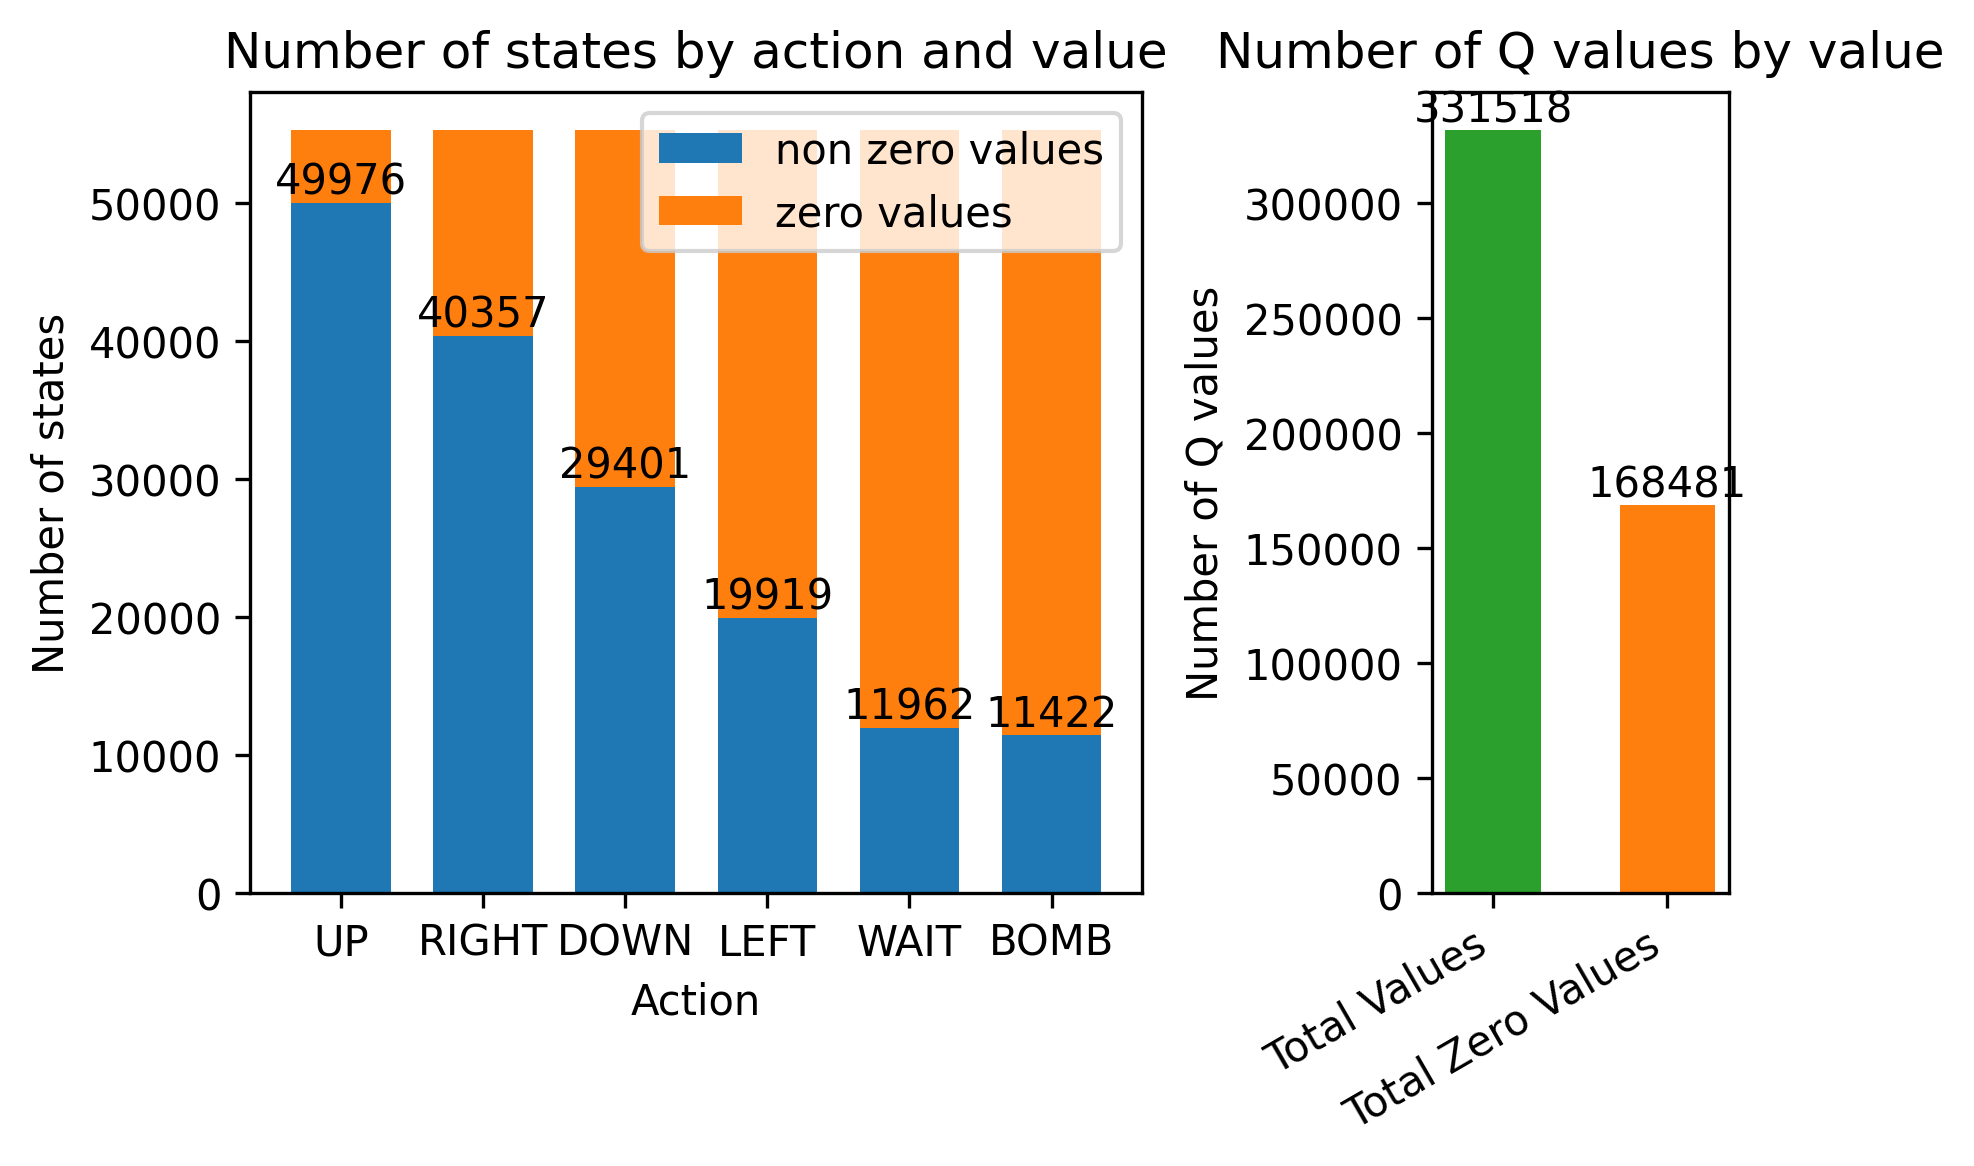
\includegraphics[width =\textwidth]{Figures/zeros.png}
	\caption{Overview of zero values in the Q table. The left Figure shows the ratio of zero to non - zero
		values per action. The right Figure shows the overall zero to non-zero ratio in the entire
		Q table.}
	\label{img:zero-values}
\end{figure}

\paragraph*{Zero values}
Our final Q table consists of 55253 states and 331518 Q values. %%%%%%%%%%%%%%%%%%%%%%%%%%%%%%%%%%%%%%%%%
A major bottleneck in the development of the agent was the lengthy training.
The majority of the last week before the submission was utilized for training.
However, this proved to not be enough as the
right chart of Figure \ref{img:zero-values} shows. About half of the Q table consists of zero
values, which means that half of the actions were never tried out.
However, the distribution of zero values is not equal among the six actions. As the left chart of Figure
\ref{img:zero-values} shows, the majority of the zero values are found in the actions
WAIT and BOMB. Specifically, these actions were executed only in 20\% of the states.
In contrast, the action UP was executed in 49976 out of the 55253 states,
or in other words in over 90\% of the states.


\subsubsection{Scenario-related performance comparison \AB}
The submitted agent exceeds the majority of the think time due to an iteration while searching for
similar states.
As the exceeding in think time isn't related to Q-Learning but to the programmatic implementation of a search function,
we perform the following experiments after replacing the iteration with a scipy function.
The result of the search function remains the same.
However, this way we are able to illustrate the performance of our Q-Learning implementation
considerating the selected hyperparameters and auxilliary rewards.


\begin{figure}[H]
	\centering
	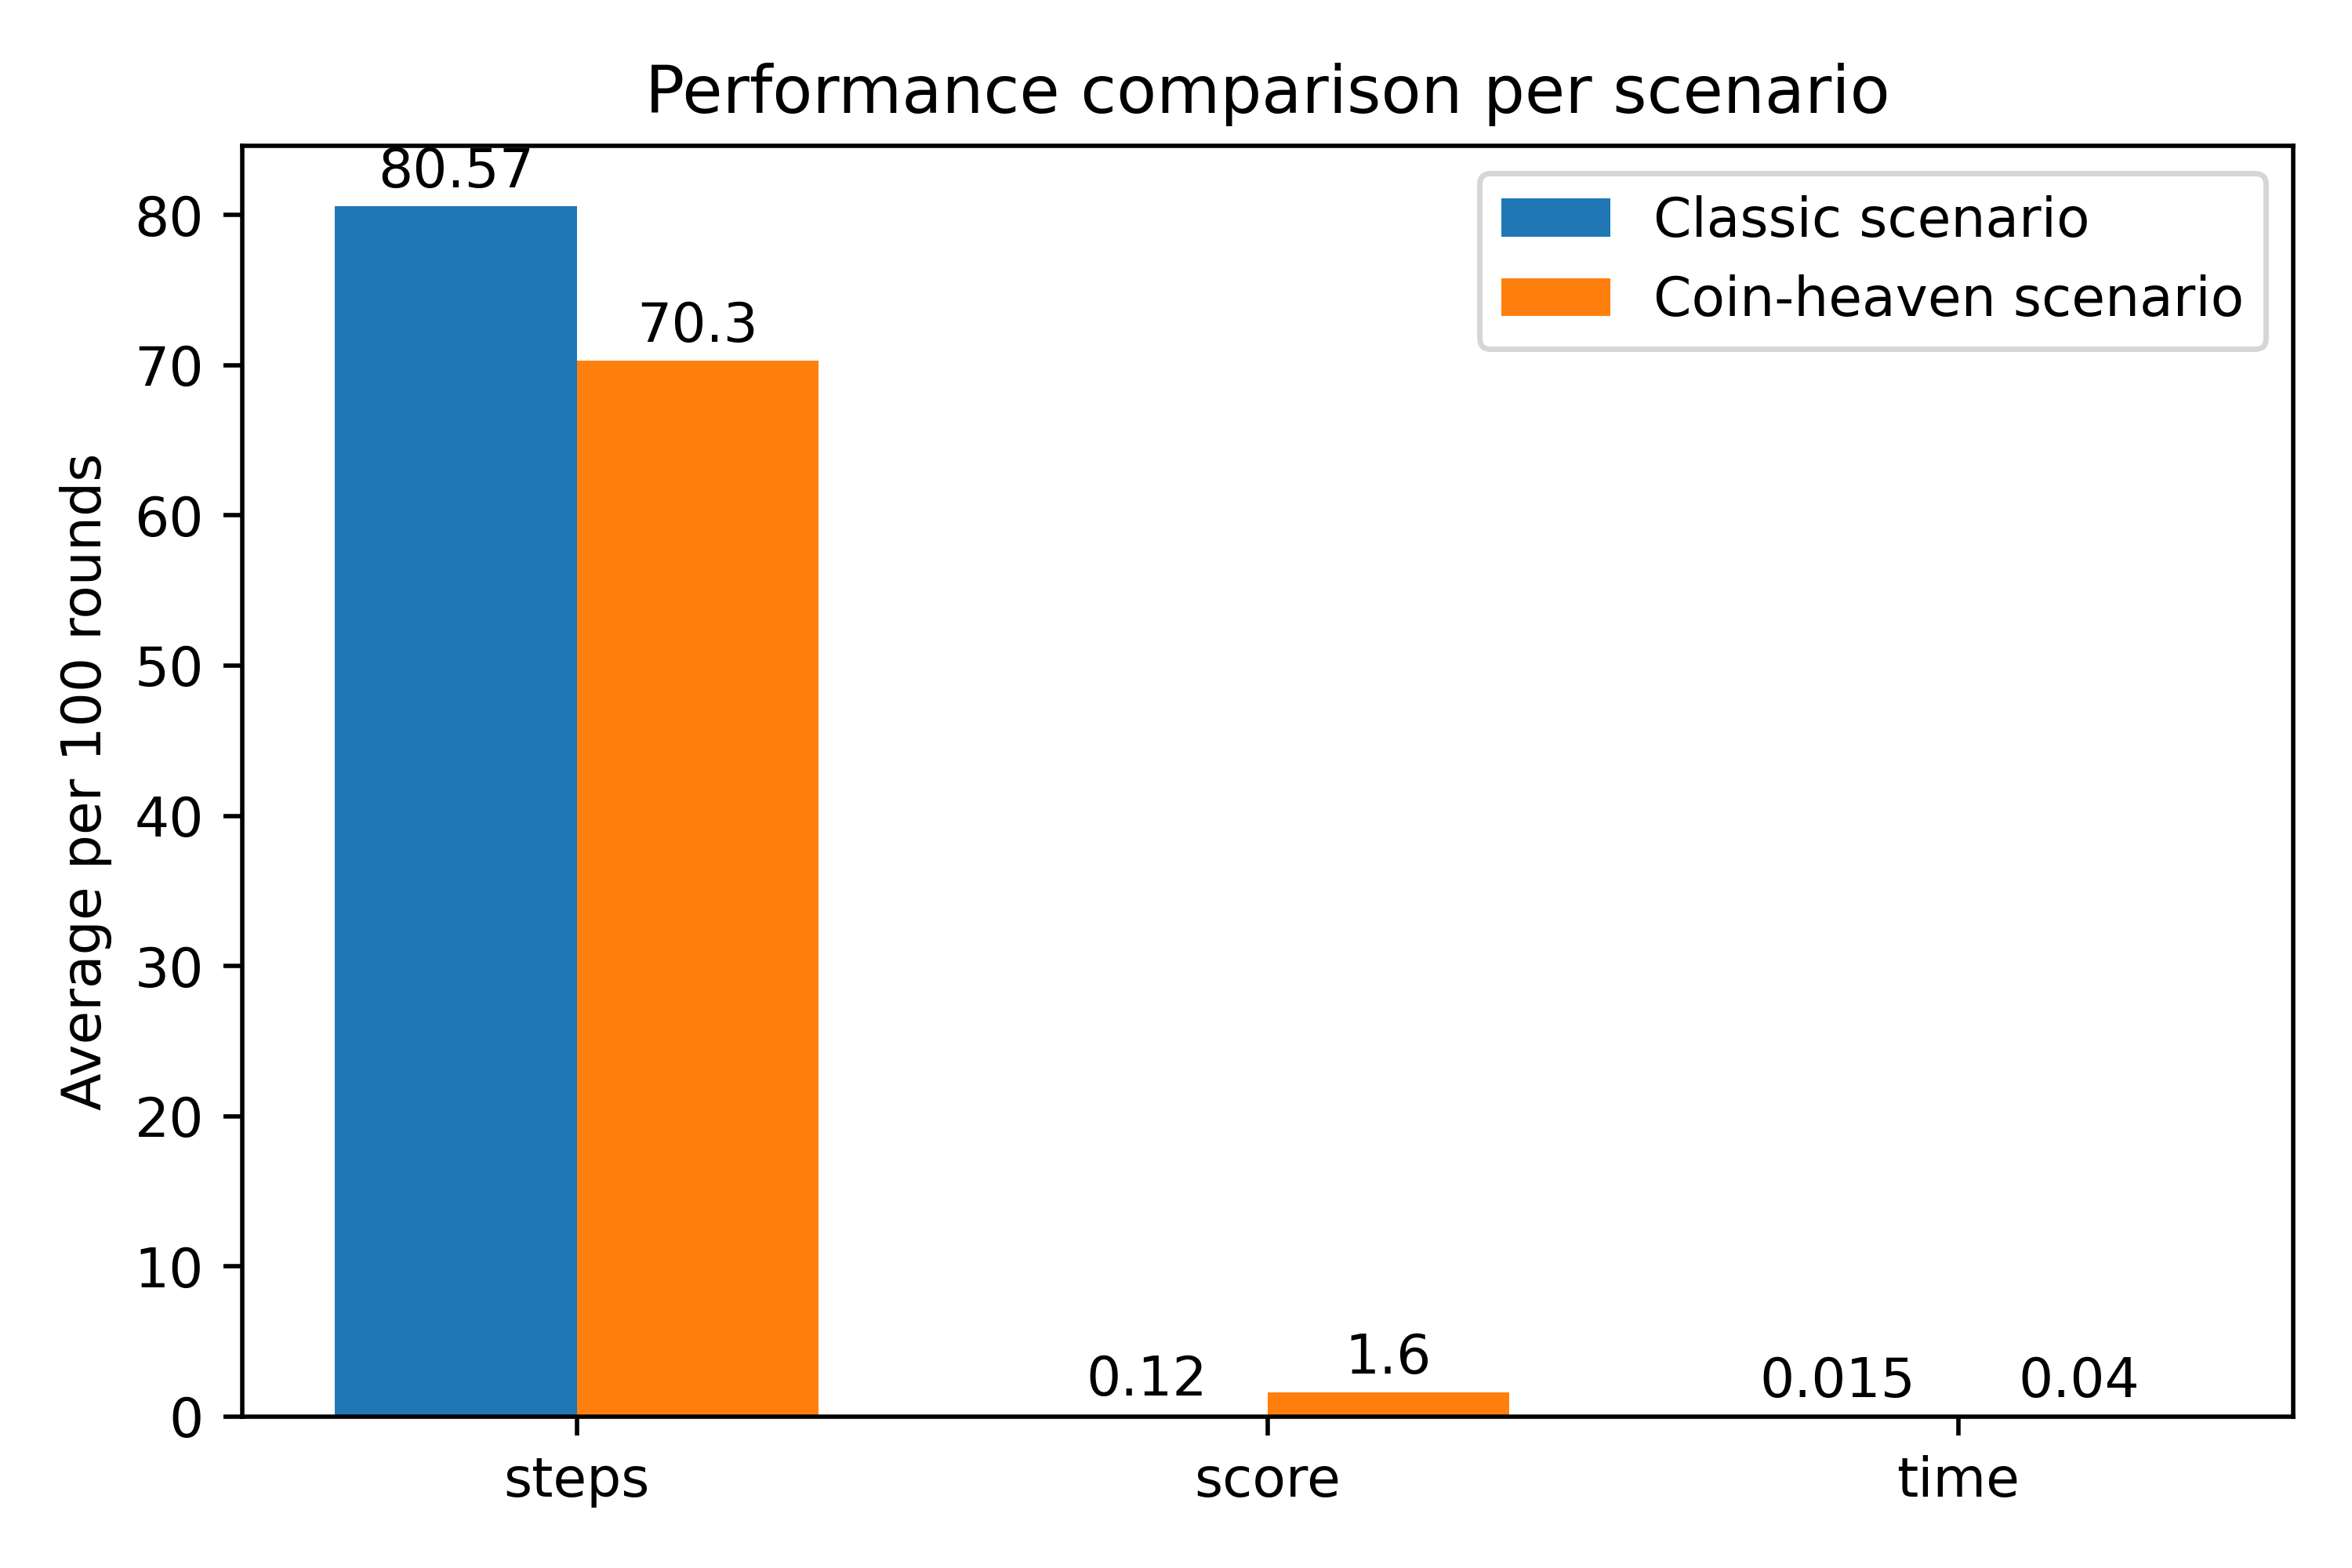
\includegraphics[scale=0.6]{Figures/metrics.png}
	\caption{Comparison of game metrics in the classic and coin-heaven scenario. The values
		correspond to an average value per round after playing for 100 rounds.}
	\label{img:metrics}
\end{figure}

Figure \ref{img:metrics} shows the game metrics in the classic and the coin-heaven
scenario. Each value equals to the average value per round after playing 100 rounds.

In the classic scenario, the agent plays on average for 80 steps. In contrast, in the
coin-heaven scenario the agent plays only for 70 steps. In both scenarios, the
average round ends way before the 400 steps are achieved. The reason lies at that
the use of a dynamic reward shaping function in combination with a high $\gamma$ hyperparameter.
A high $\gamma$ emphasizes future rewards, which incentivizes the agent to collect a high cumulative ?? reward
over the round. However, the dynamic reward shaping function reduces the reward by the time step,
to incentivize the agent to finish the round fast. Therefore, the agent is incentivized to end the
round early to maximize its rewards, which is clearly the case in both scenarios.

In the coin-heaven scenario, the average score equals to 1.6 points which is by 13 times higher.
While in the classic scenario,
the agents earns 0.12 points. As the agent was primarily trained in the coin-heaven scenario, the Q values of
the states of the coin-heaven scenario converged better than the Q values of the classic scenario.

The think time in the coin-heaven scenario is by 2.5 times higher than in the classic scenario.
The think time at seen states is XX??. For unseen states, the agent searches for the most similar seen state
in the Q table and chooses its best action. ????


\begin{figure}[H]
	\centering
	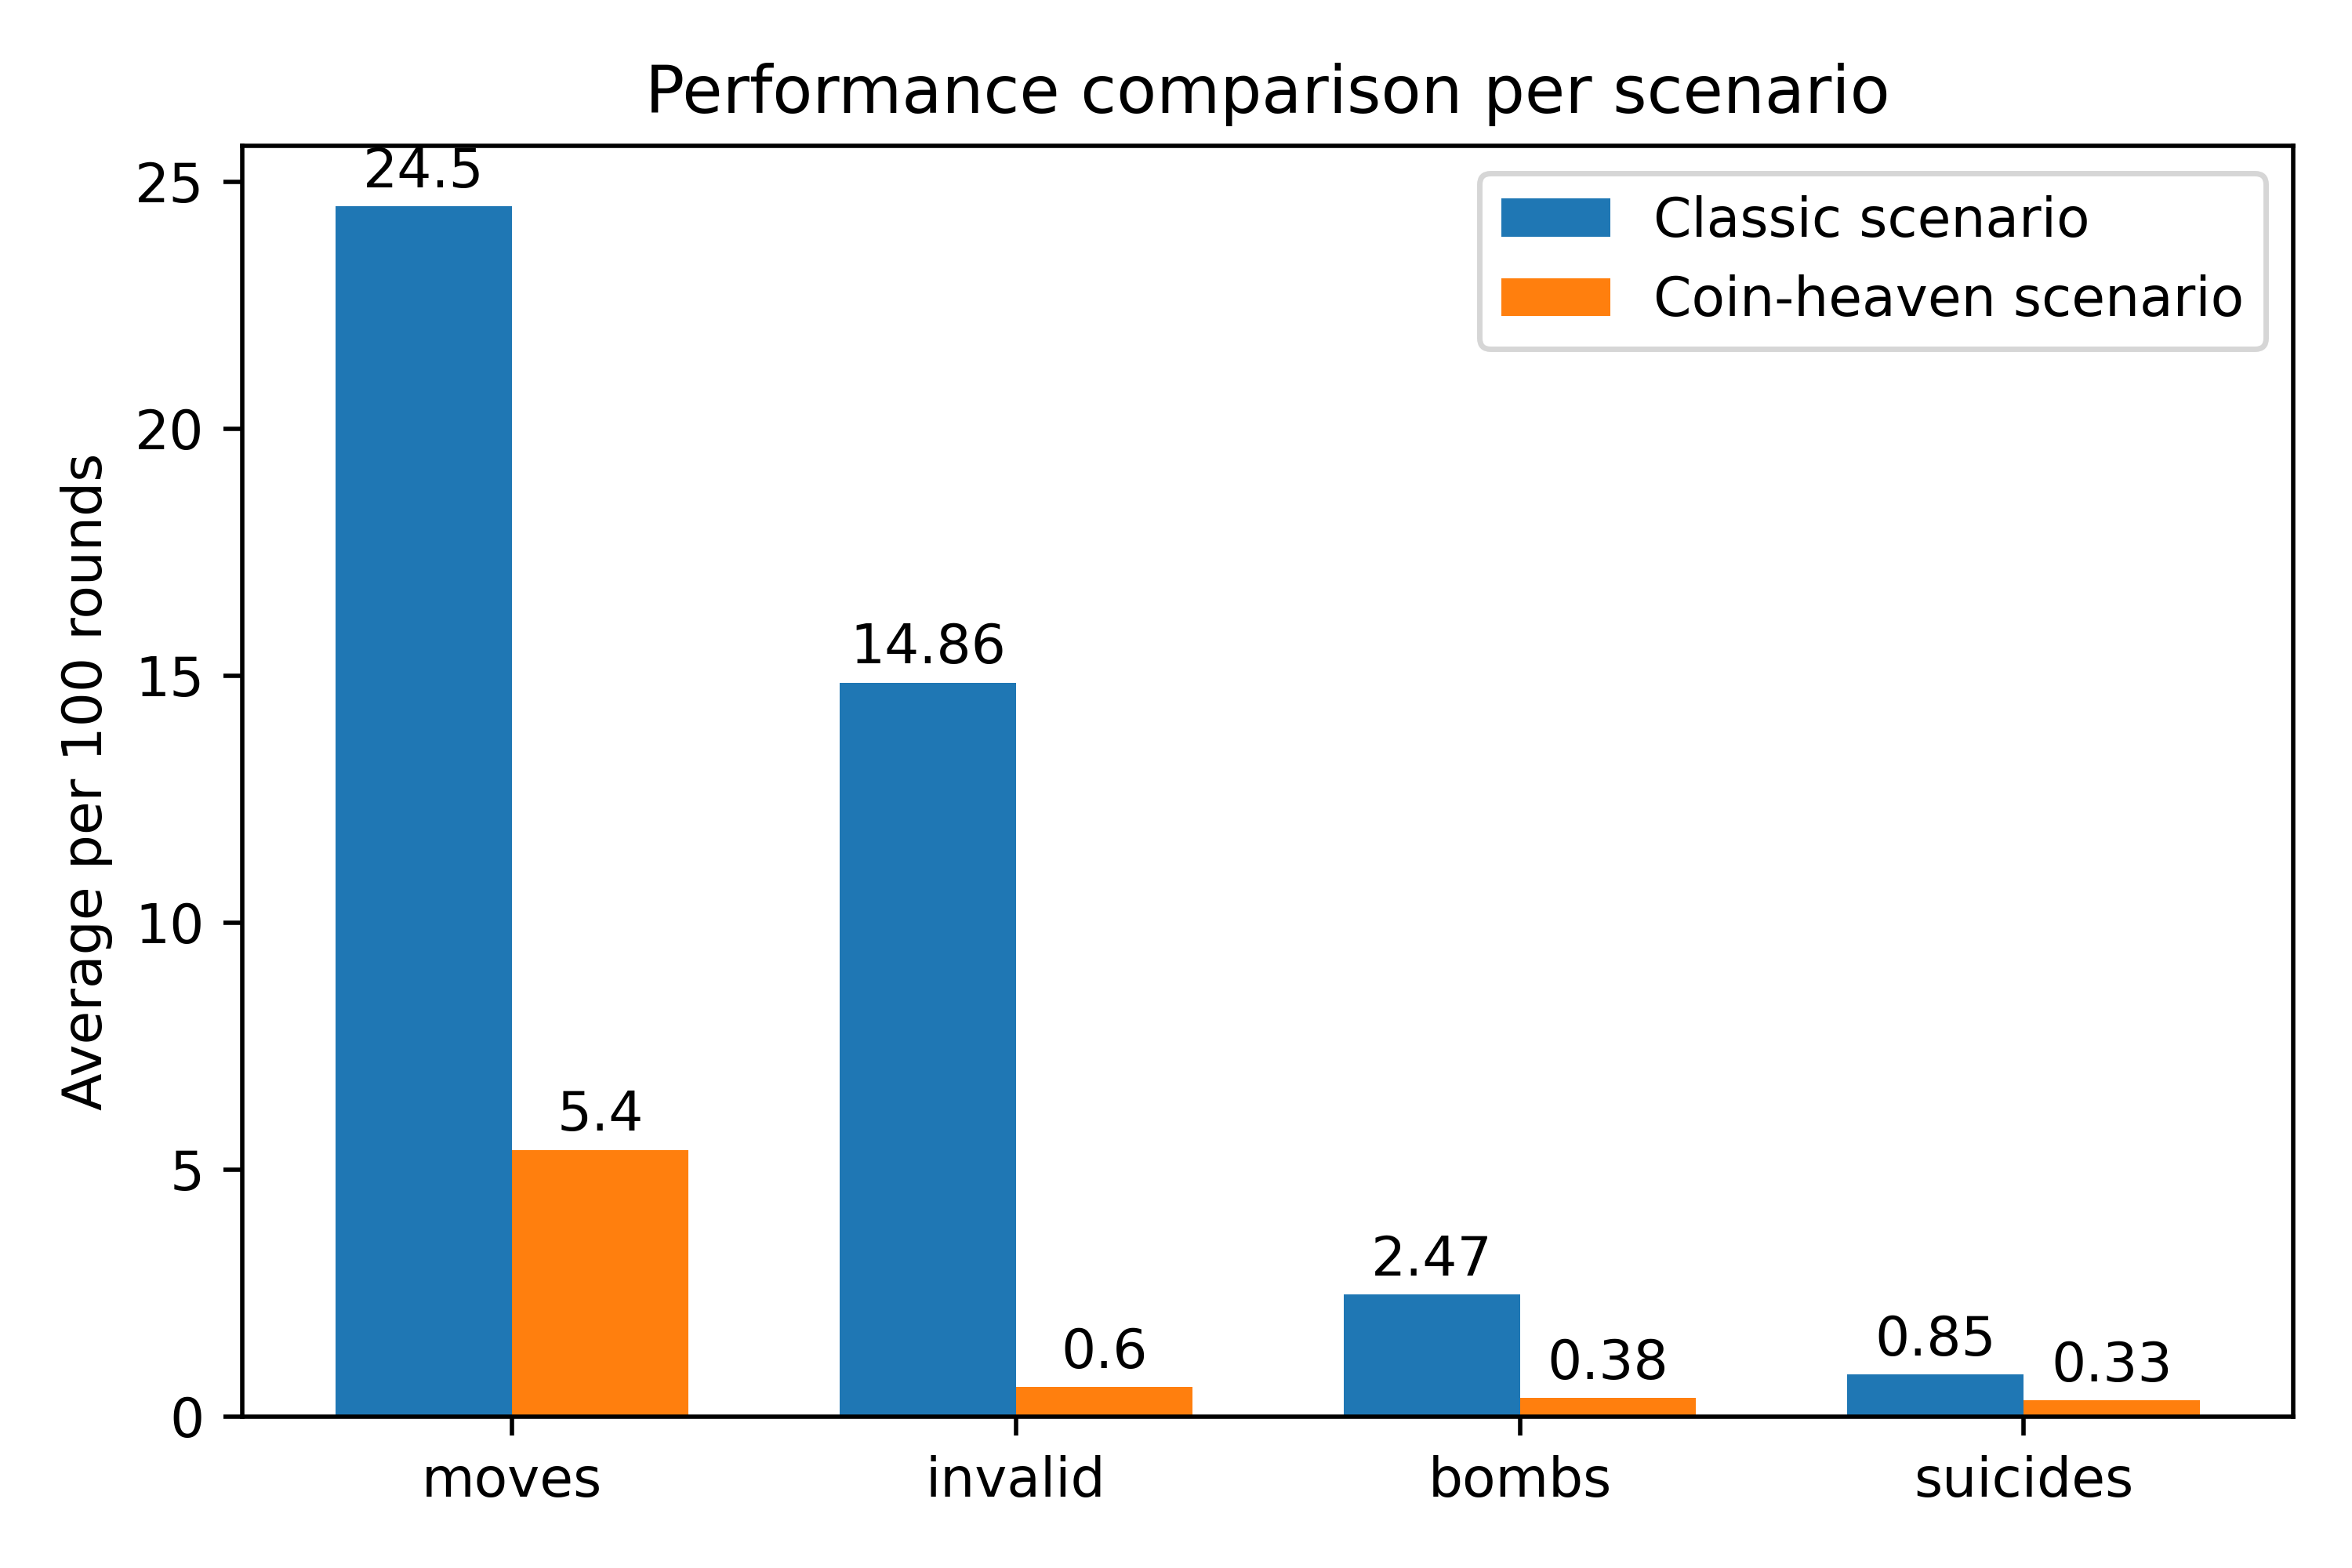
\includegraphics[scale=0.6]{Figures/game.png}
	\caption{Comparison of performance in the classic and coin-heaven scenario. The values
		correspond to an average value per round after playing for 100 rounds.}
	\label{img:game}
\end{figure}

Figure \ref{img:game} shows the effect of the moves in the classic and the coin-heaven
scenario.


Over all four metrics the classic scenario contains consistently higher values.
This indicates the worst performance in comparison to the coin-heaven scenario, which
aligns with our focus on training in the coin-heaven scenario.
This observation becomes even more obvious when considering bad actions such as invalid actions and suicides.
In the coin-heaven scenario the agent chooses on average 24 times more invalid actions and performs 2.5 times
more suicides.

In the classic scenario, as the agent is less cautious with its moves, its performs on average 24.5 moves per round.
The ratio is 5x.???? what are moves

Surprisingly, the agent places 6 times more bombs in the classic scenario. Despite the shorter training time,
the beneficial action is selected way more times than in the coin-heaven scenario. Given that there are less
crates and opponents in the coin-heaven scenario than in the classic scenario, the auxilliary rewards incentivized
the use of bombs in the classic scenario. While 2.4 bombs are certainly not enough to win the round,
the bomb ratio between the two scenarios shows that the rewards give the right incentives. The main issue remains
the long training time until convergence.


Overall, the agent shows better performance in the coin-heaven scenario than in
the classic scenario. The performance is consistently better over all metrics except the time.
The longer training time resulted into more Q values closer to convergence. Nevertheless,
we observe good agent behavior in both scenarios, such as a low number of invalid actions and more bomb placing in
the scenario with crates and opponents.


\subsubsection{Task-related performance comparison}
\paragraph{Task 1 \tiny Sven Zelch}

In Task 1 an agent is supposed to collect all the coins in the coin-heaven scenario, where no other agents and no crates exists.


\begin{figure}[h]
	\centering
	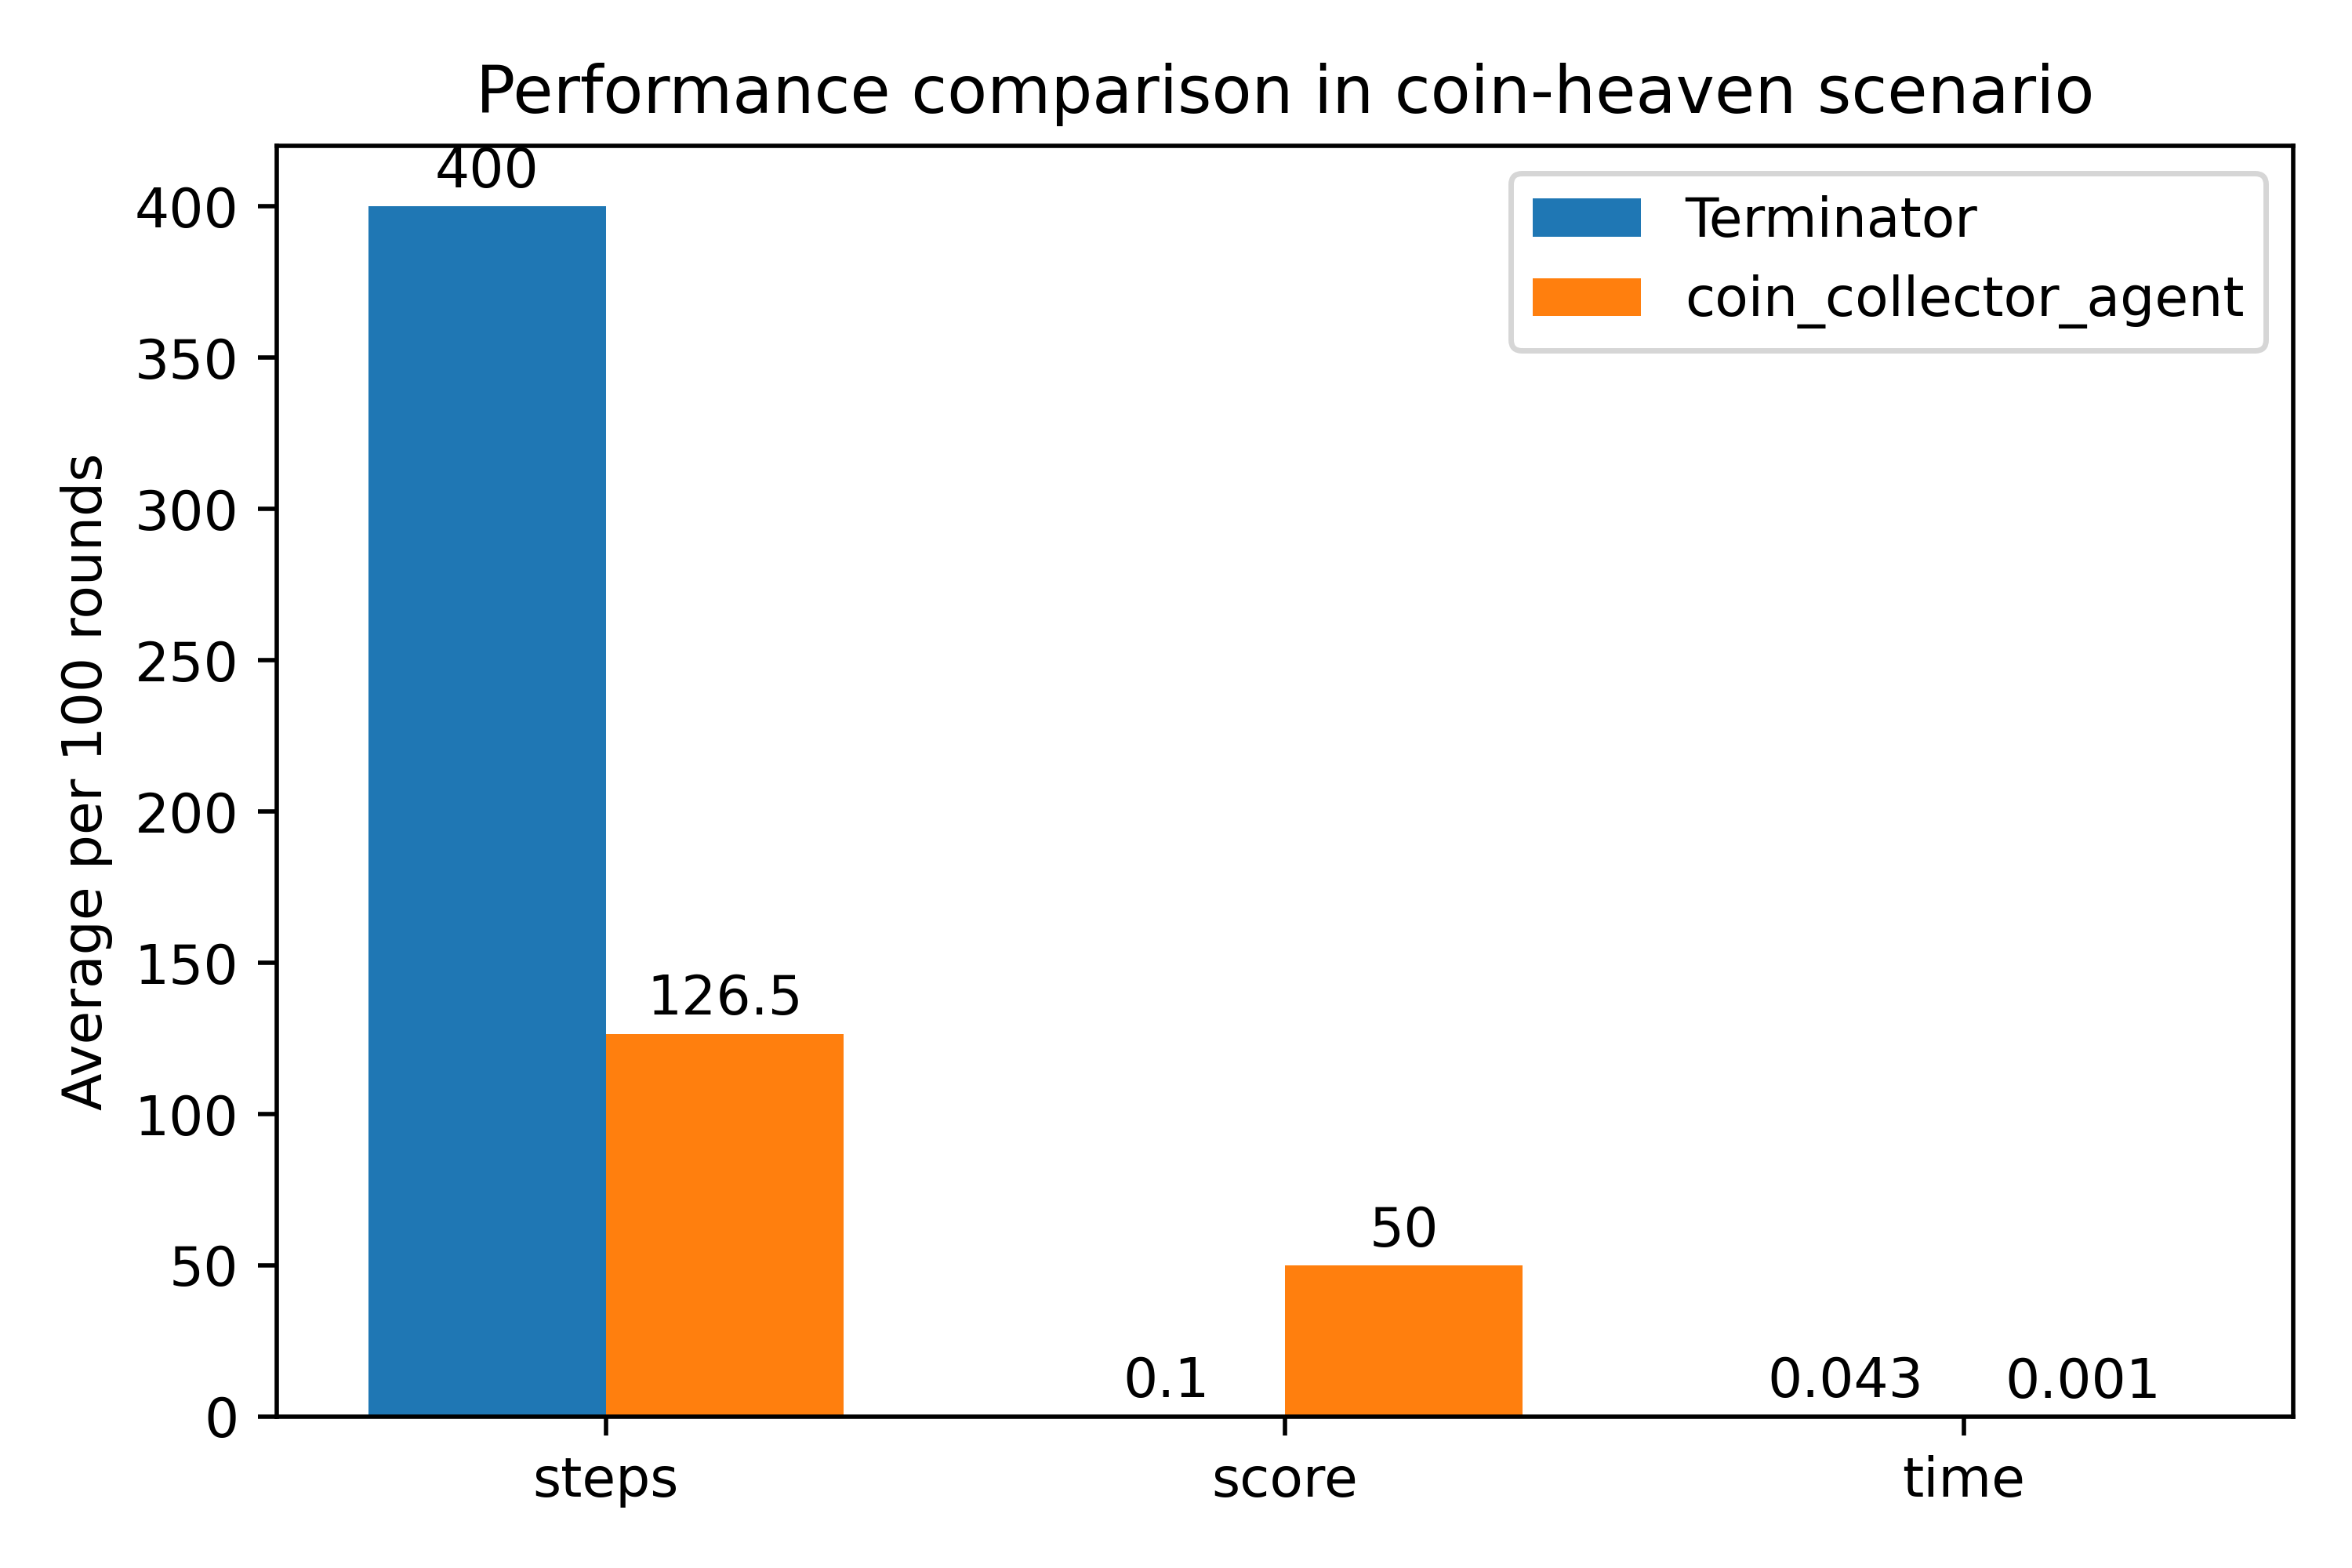
\includegraphics[scale=0.6]{Figures/Task1.png}
	\caption{Performance comparison Terminator and coin\_collector\_agent in coin-heaven scenario.}
	\label{img:Task1}
\end{figure}

Figure \ref{img:Task1} compares the performance of our agent with the coin\_collector\_agent for Task 1.
The coin\_collector\_agent shows an ideal scenario of how our agent should behave he reaches a score of 50 in all 100 games played, which means he always collects all 50 coins in the coin-heaven scenario, because it is the only way he can increase his score and each collected coin increases its score by one.
Our agent struggles to collect the coins within the given time of 400 steps.
In fact he only collects 1 coin every 10 games.
Watching the game with GUI on we can see the agent is waiting a lot.
This issue occurred before where the time it takes for the agent to chose an action was greater than 0.5 seconds and the agent was forced by the game to wait.
We are unsure what causes this issue this time around.
%It could be caused by a lot of invalid actions as Task 2 suggests.

\paragraph{Task 2 \tiny Sven Zelch}

Task 2 is similar to Task 1, but this time some coins are hidden under crates. The crates need to be blown up first before the agent can collects the coins. We used the classic scenario without other agents for this task.

\begin{figure}[H]

	\begin{subfigure}{\textwidth}
		\centering
		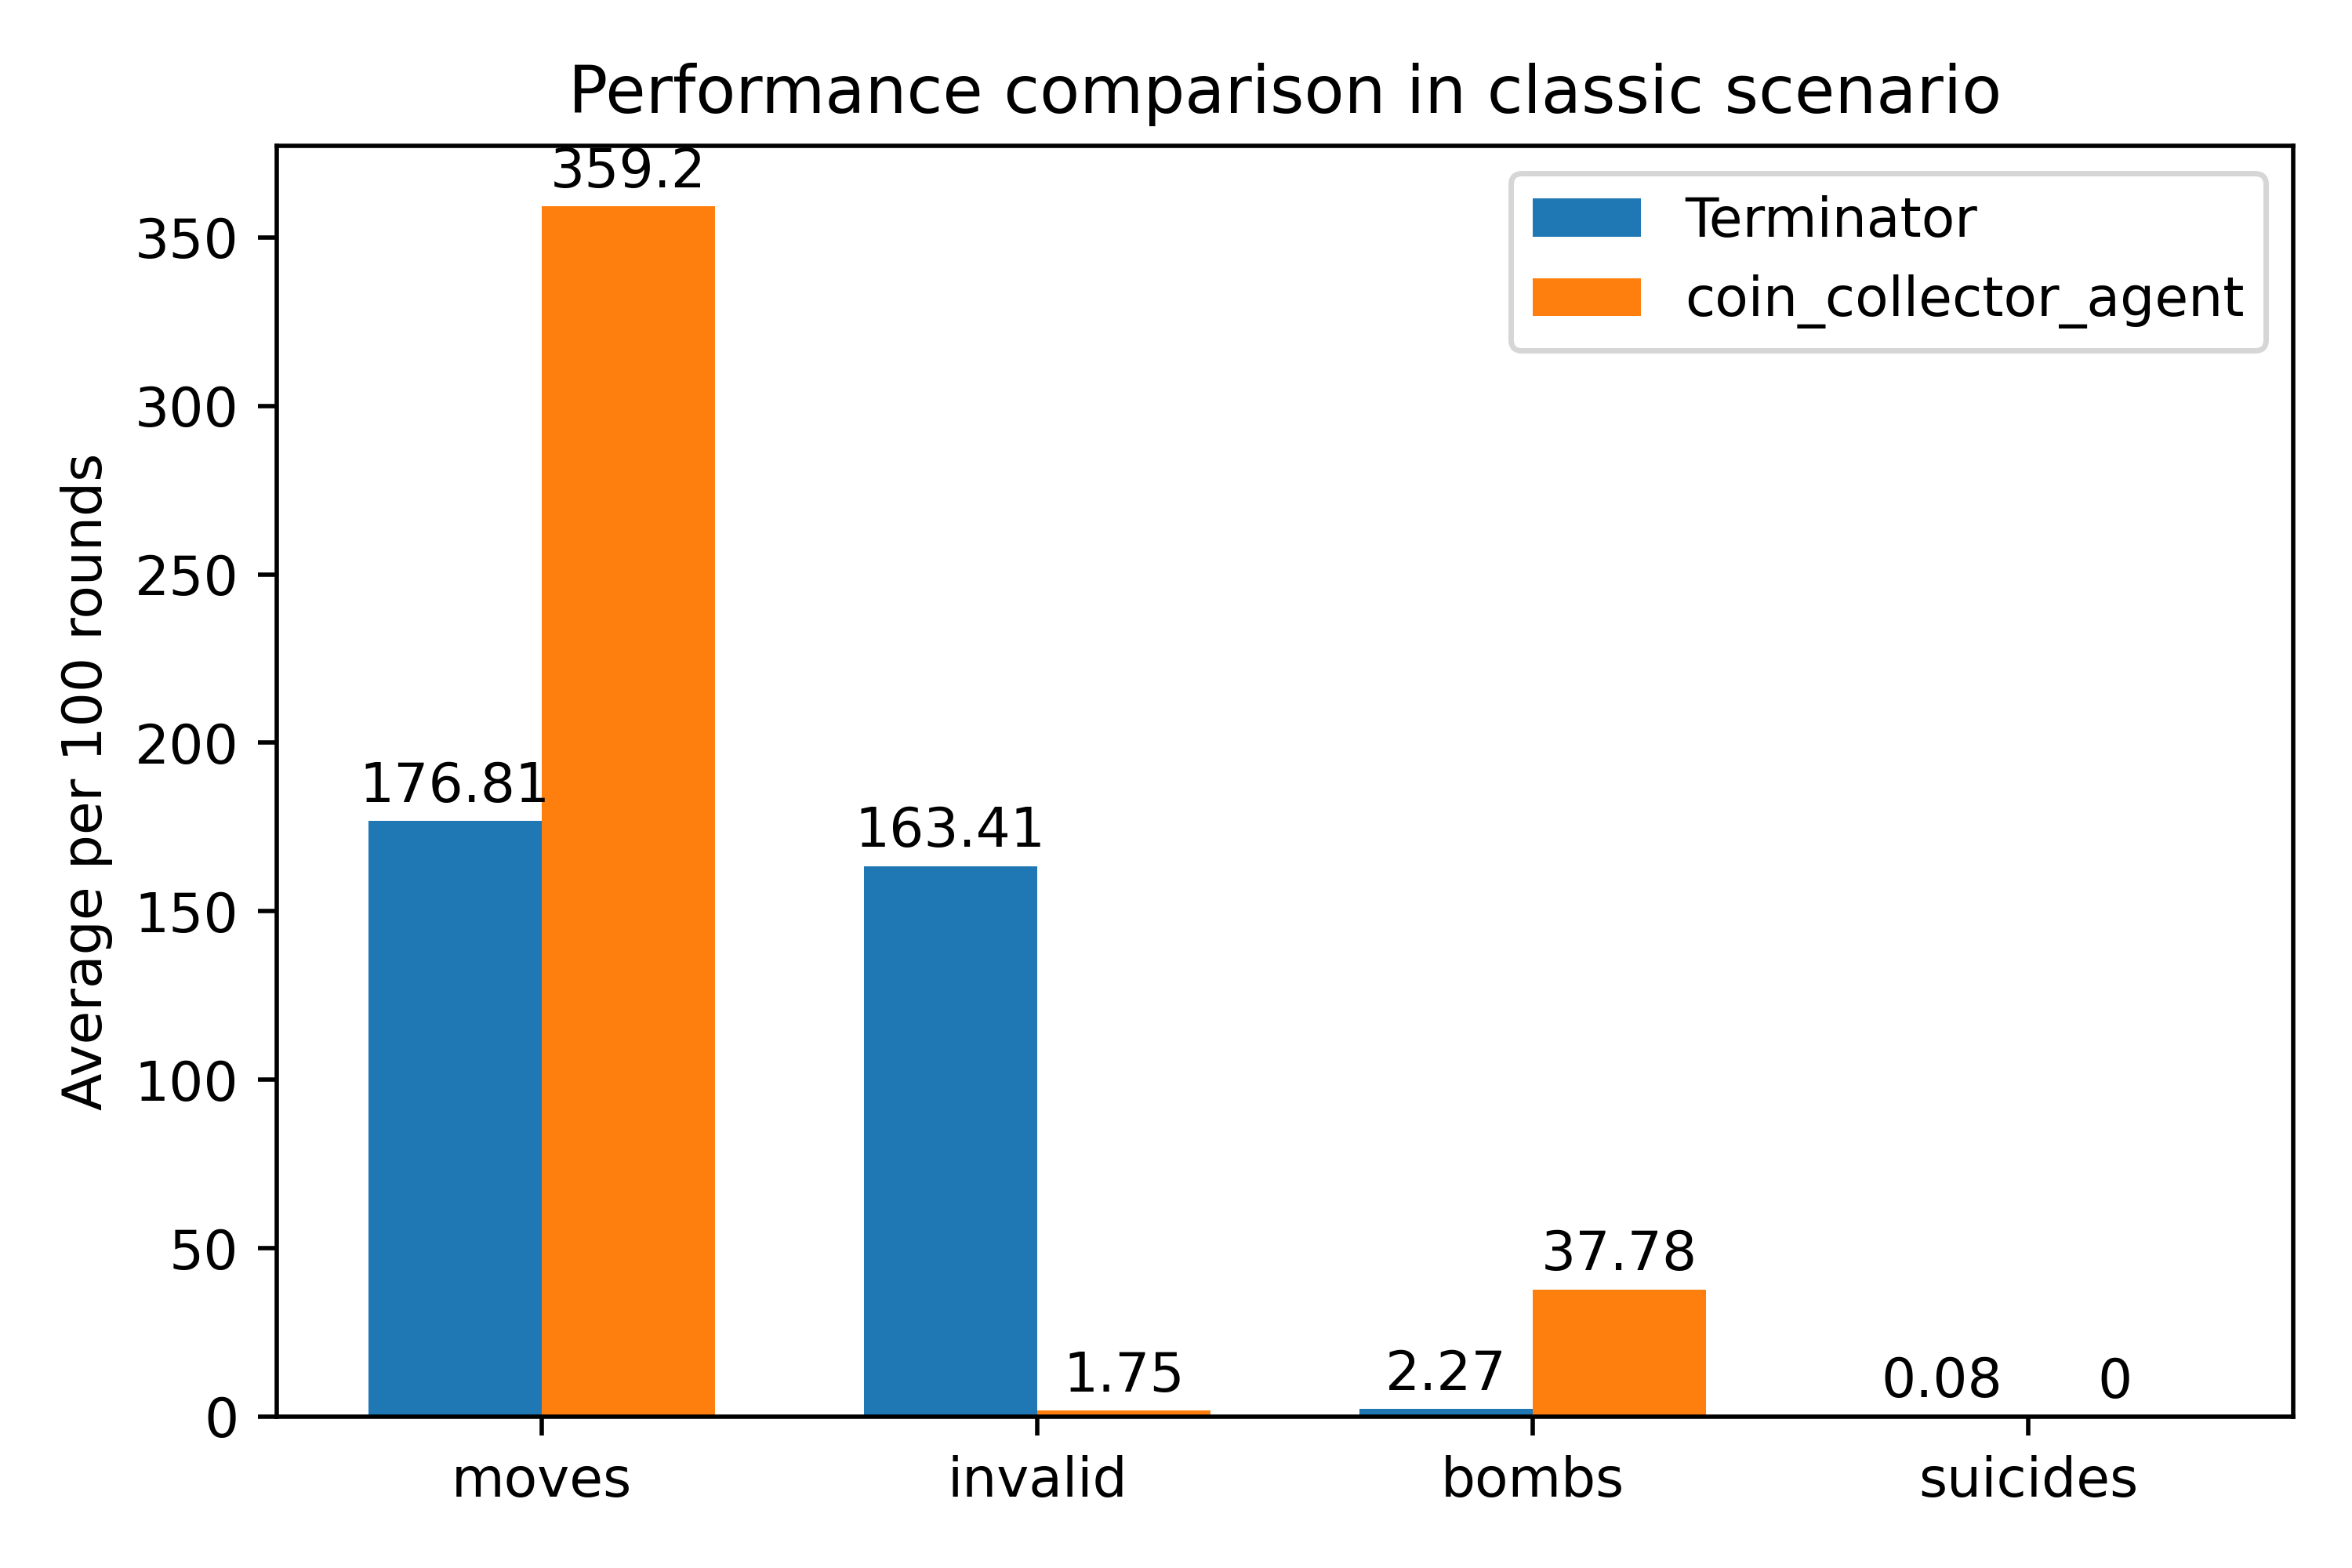
\includegraphics[scale=0.6]{Figures/Task2-1.png}
		\caption{Performance comparison Terminator and coin\_collector\_agent moves}
		\label{img:Task2-1}
	\end{subfigure}


	\begin{subfigure}{\textwidth}
		\centering
		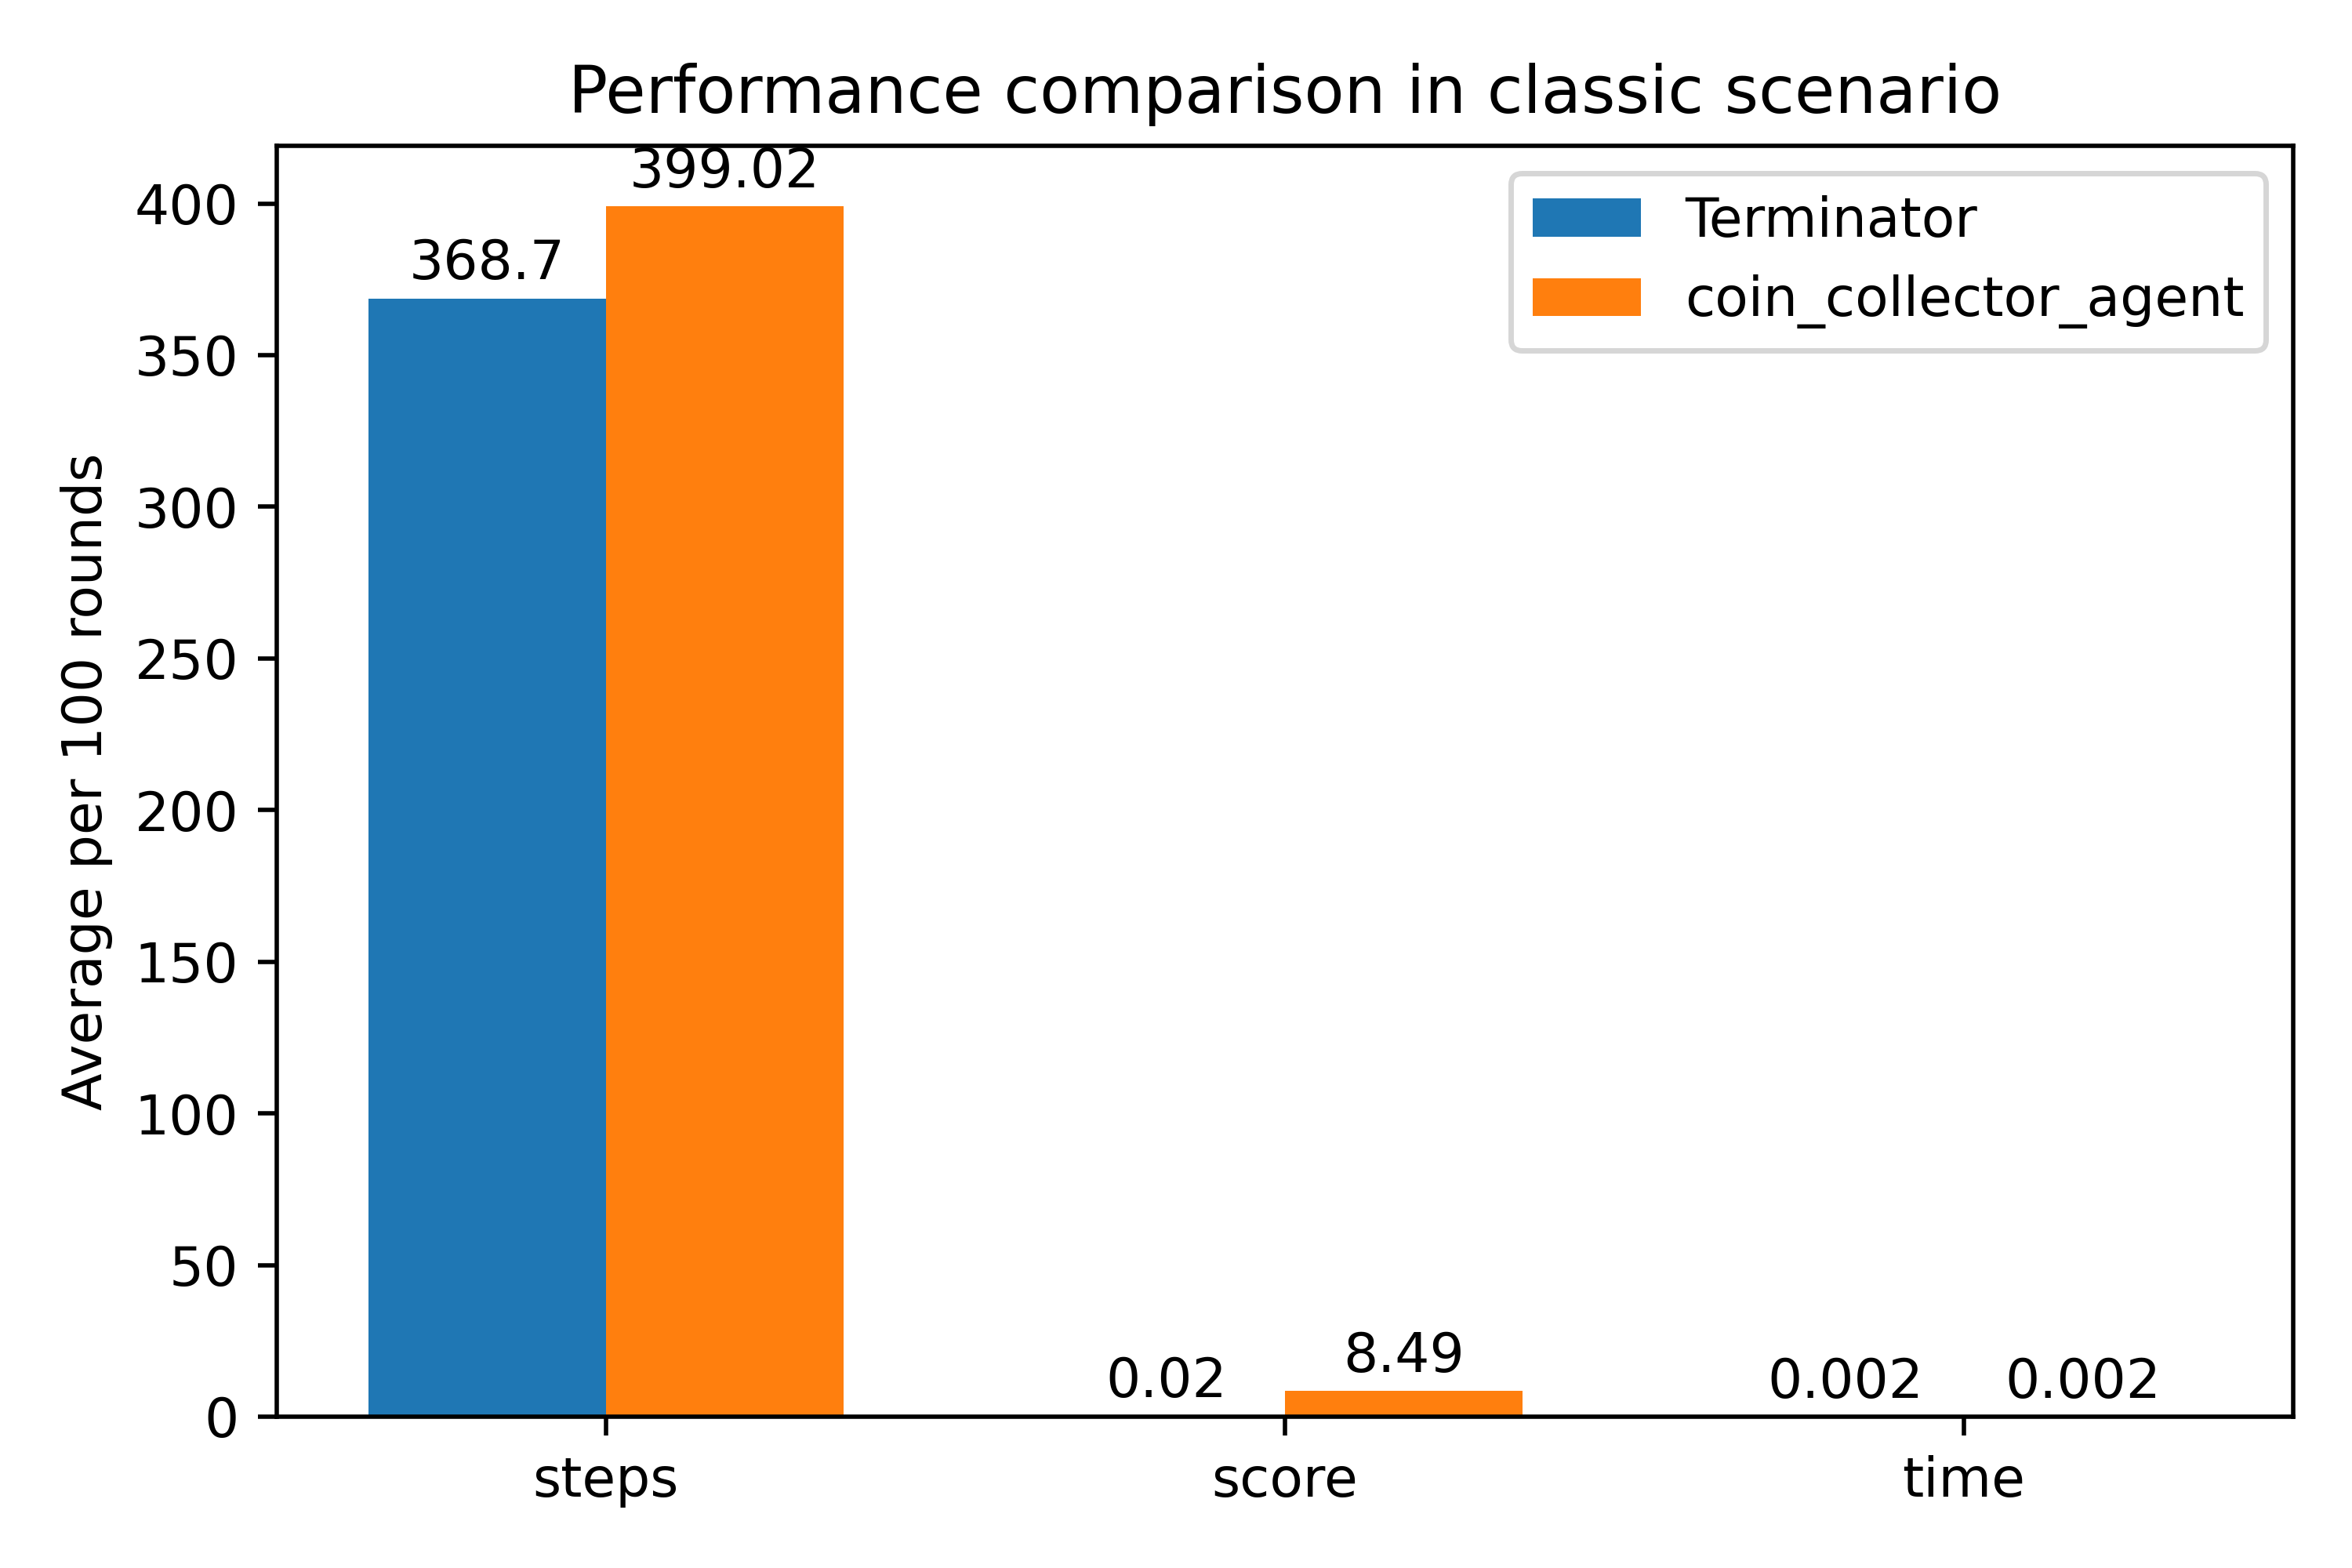
\includegraphics[scale=0.6]{Figures/Task2-2.png}
		\caption{Performance comparison Terminator and coin\_collector\_agent game}
		\label{img:Task2-2}
	\end{subfigure}

	\caption{Performance comparison Terminator and coin\_collector\_agent in classic scenario without opponents}
	\label{img:Task2}

\end{figure}

Figure \ref{img:Task2-1} and \ref{img:Task2-2} compare the performance of our agent with the coin\_collector\_agent for Task 2.
Again the coin\_collector\_agent performs way better than the Terminator, especially score wise.
Also it does about two times more moves than our agent and if we only count valid moves:
$(359.2- 1.75) / (176.81 - 163.41) \approx 27$
times more valid moves.
The issue in Task 1 could also be caused by a lot of invalid actions, which look like the agent is waiting actions from the GUI perspective.
As well as the limited amount of bombs Terminator drops is caused by the limited small amount of valid actions, about 13 per round, it takes.
A good thing about our agent is that he only suicides 8 times in 100 games which is worse than the coin\_collector\_agent, but still a great result nevertheless.
Both agents seem to struggle to find all the coins in 400 steps.
Terminator has a lower step count, because he suicides himself sometimes.
Something really interesting here is that both agents take approximately the same time to chose an action.
Particularly comparing the result from Terminator with them from Figure \ref{img:Task1} a high reduce in time to chose an action can be seen.
This is probably caused by the agent being mostly trained in the classic scenario.

\paragraph{Task 3 \tiny Sven Zelch}

In this Task the agent should additionally to collecting coins also try to hunt and blow up an opposite agent.

\begin{figure}[H]

	\begin{subfigure}{\textwidth}
		\centering
		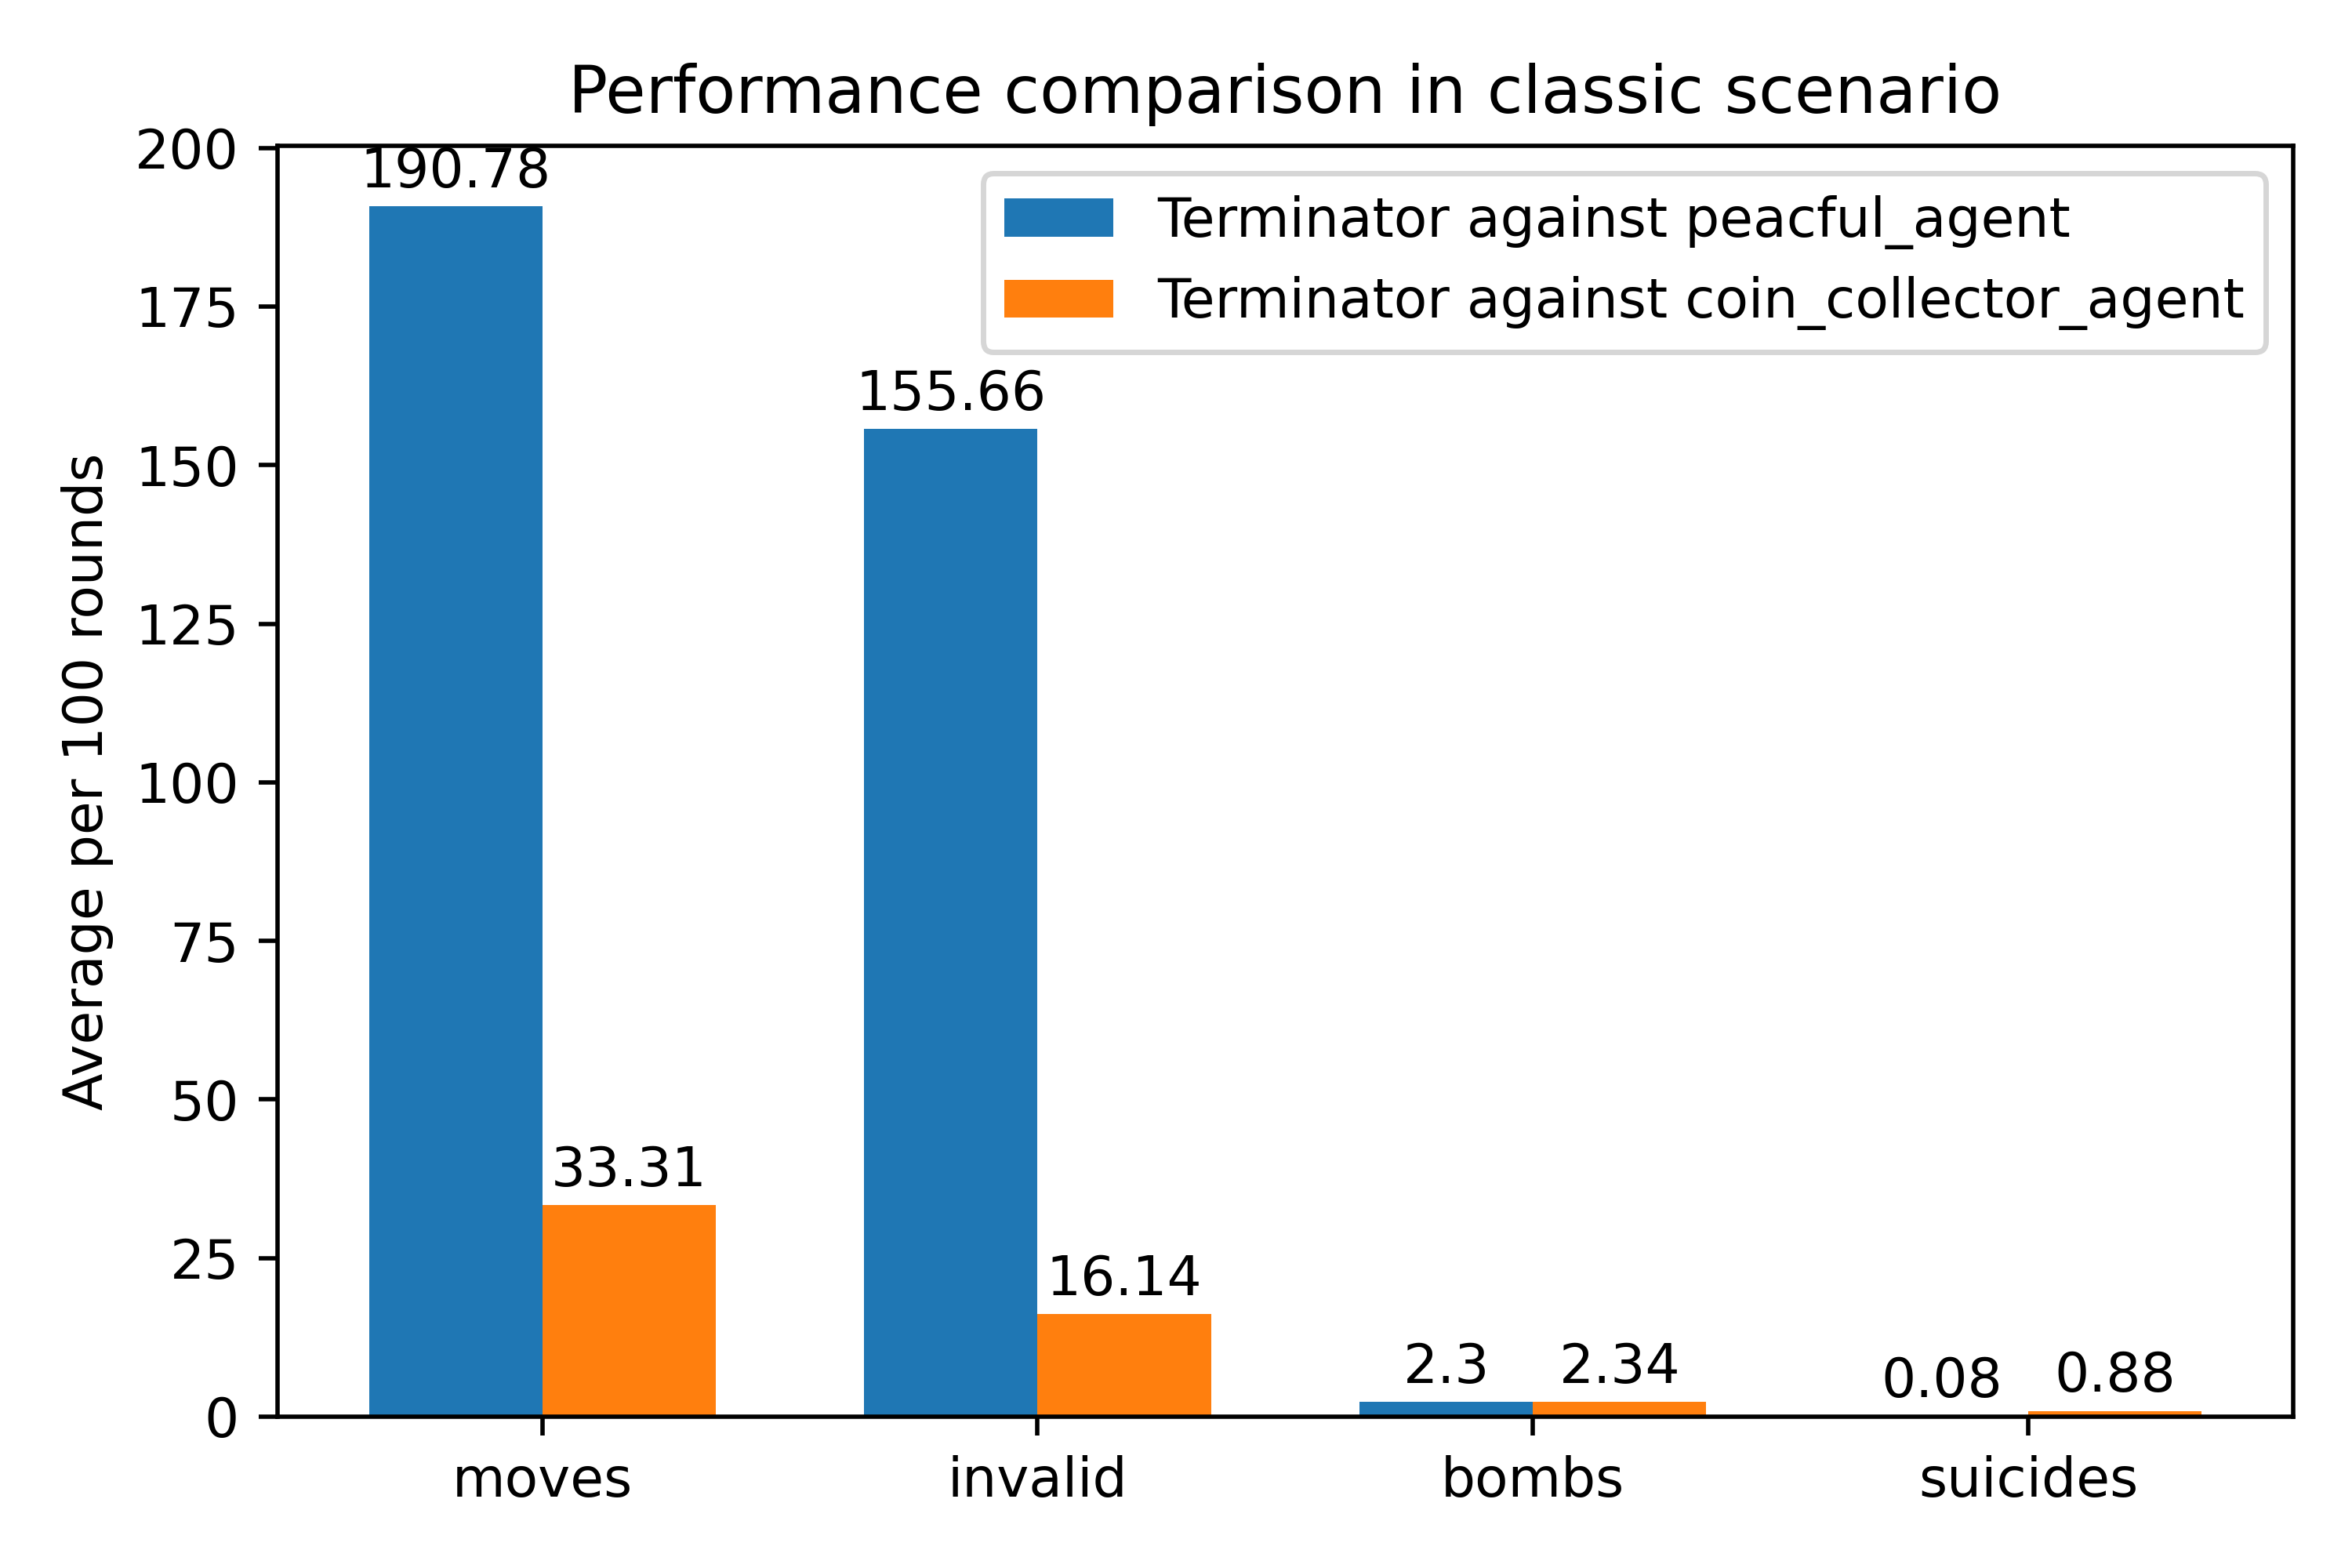
\includegraphics[scale=0.6]{Figures/Task3-1.png}
		\caption{Performance comparison Terminator against peaceful\_agent and Terminator against coin\_collector\_agent moves}
		\label{img:Task3-1}
	\end{subfigure}

	\begin{subfigure}{\textwidth}
		\centering
		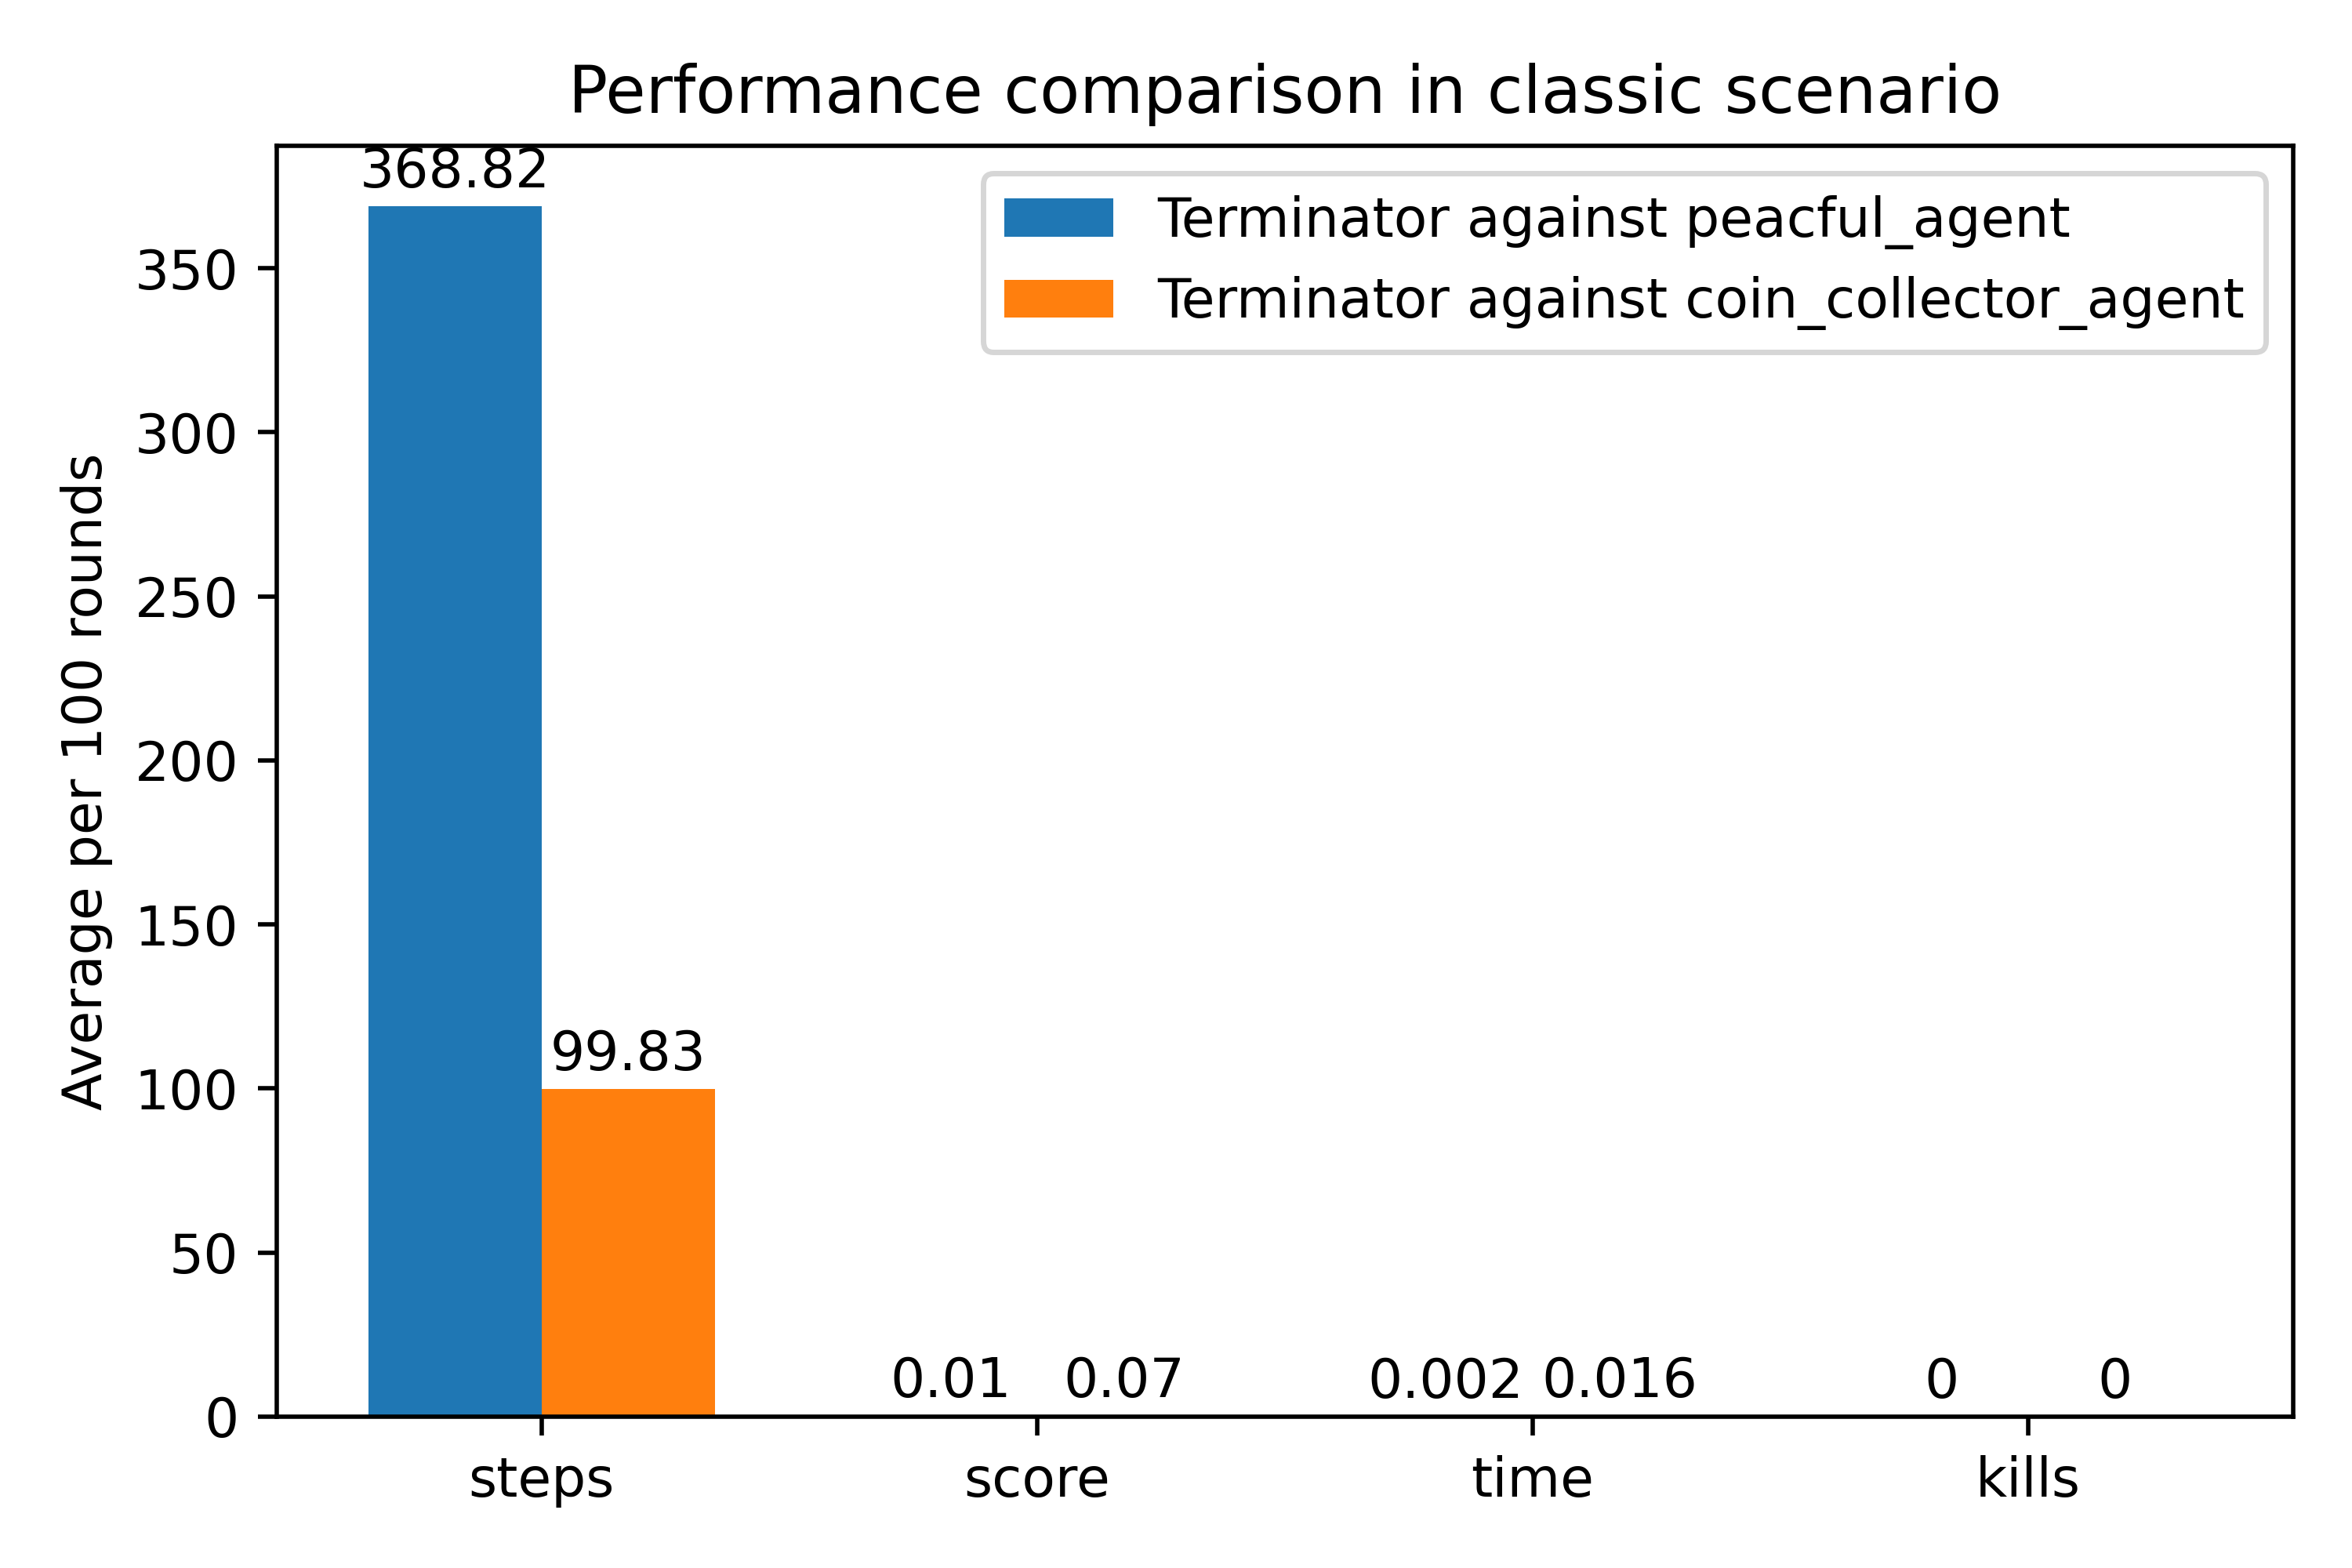
\includegraphics[scale=0.6]{Figures/Task3-2.png}
		\caption{Performance comparison Terminator against peaceful\_agent and Terminator against coin\_collector\_agent game}
		\label{img:Task3-2}
	\end{subfigure}

	\caption{Performance comparison Terminator against peaceful\_agent and Terminator against coin\_collector\_agent}
	\label{img:Task3}

\end{figure}

Figure \ref{img:Task3-1} and \ref{img:Task3-2} compare the performance of our agent Terminator against the peaceful\_agent, who does not drop bombs and against the coin\_collector\_agent who only drops bombs to destroy crates.
The peaceful\_agent seems to have barley any influence on the agent, because results of the match against the peaceful against are similar to the results of Figure \ref{img:Task2-1} and \ref{img:Task2-2}.
Interestingly however is that the coin\_collector\_agent has a drastic effect on Terminators performance.
The suicide rate is 11 times higher, even tough he drops the same amount of bombs.
As a result of that he performs less moves, but about half his actions are valid actions compared to a fifth.
Regardless of less rounds played the score is a bit better, but that is probably caused by small sample size.
In both cases Terminator failed to kill his opponent.

\paragraph{Task 4 \tiny Sven Zelch}

The agent competes against one ore more agents for the highest score in a classic Bomberman game.

\begin{figure}[H]

	\begin{subfigure}{\textwidth}
		\centering
		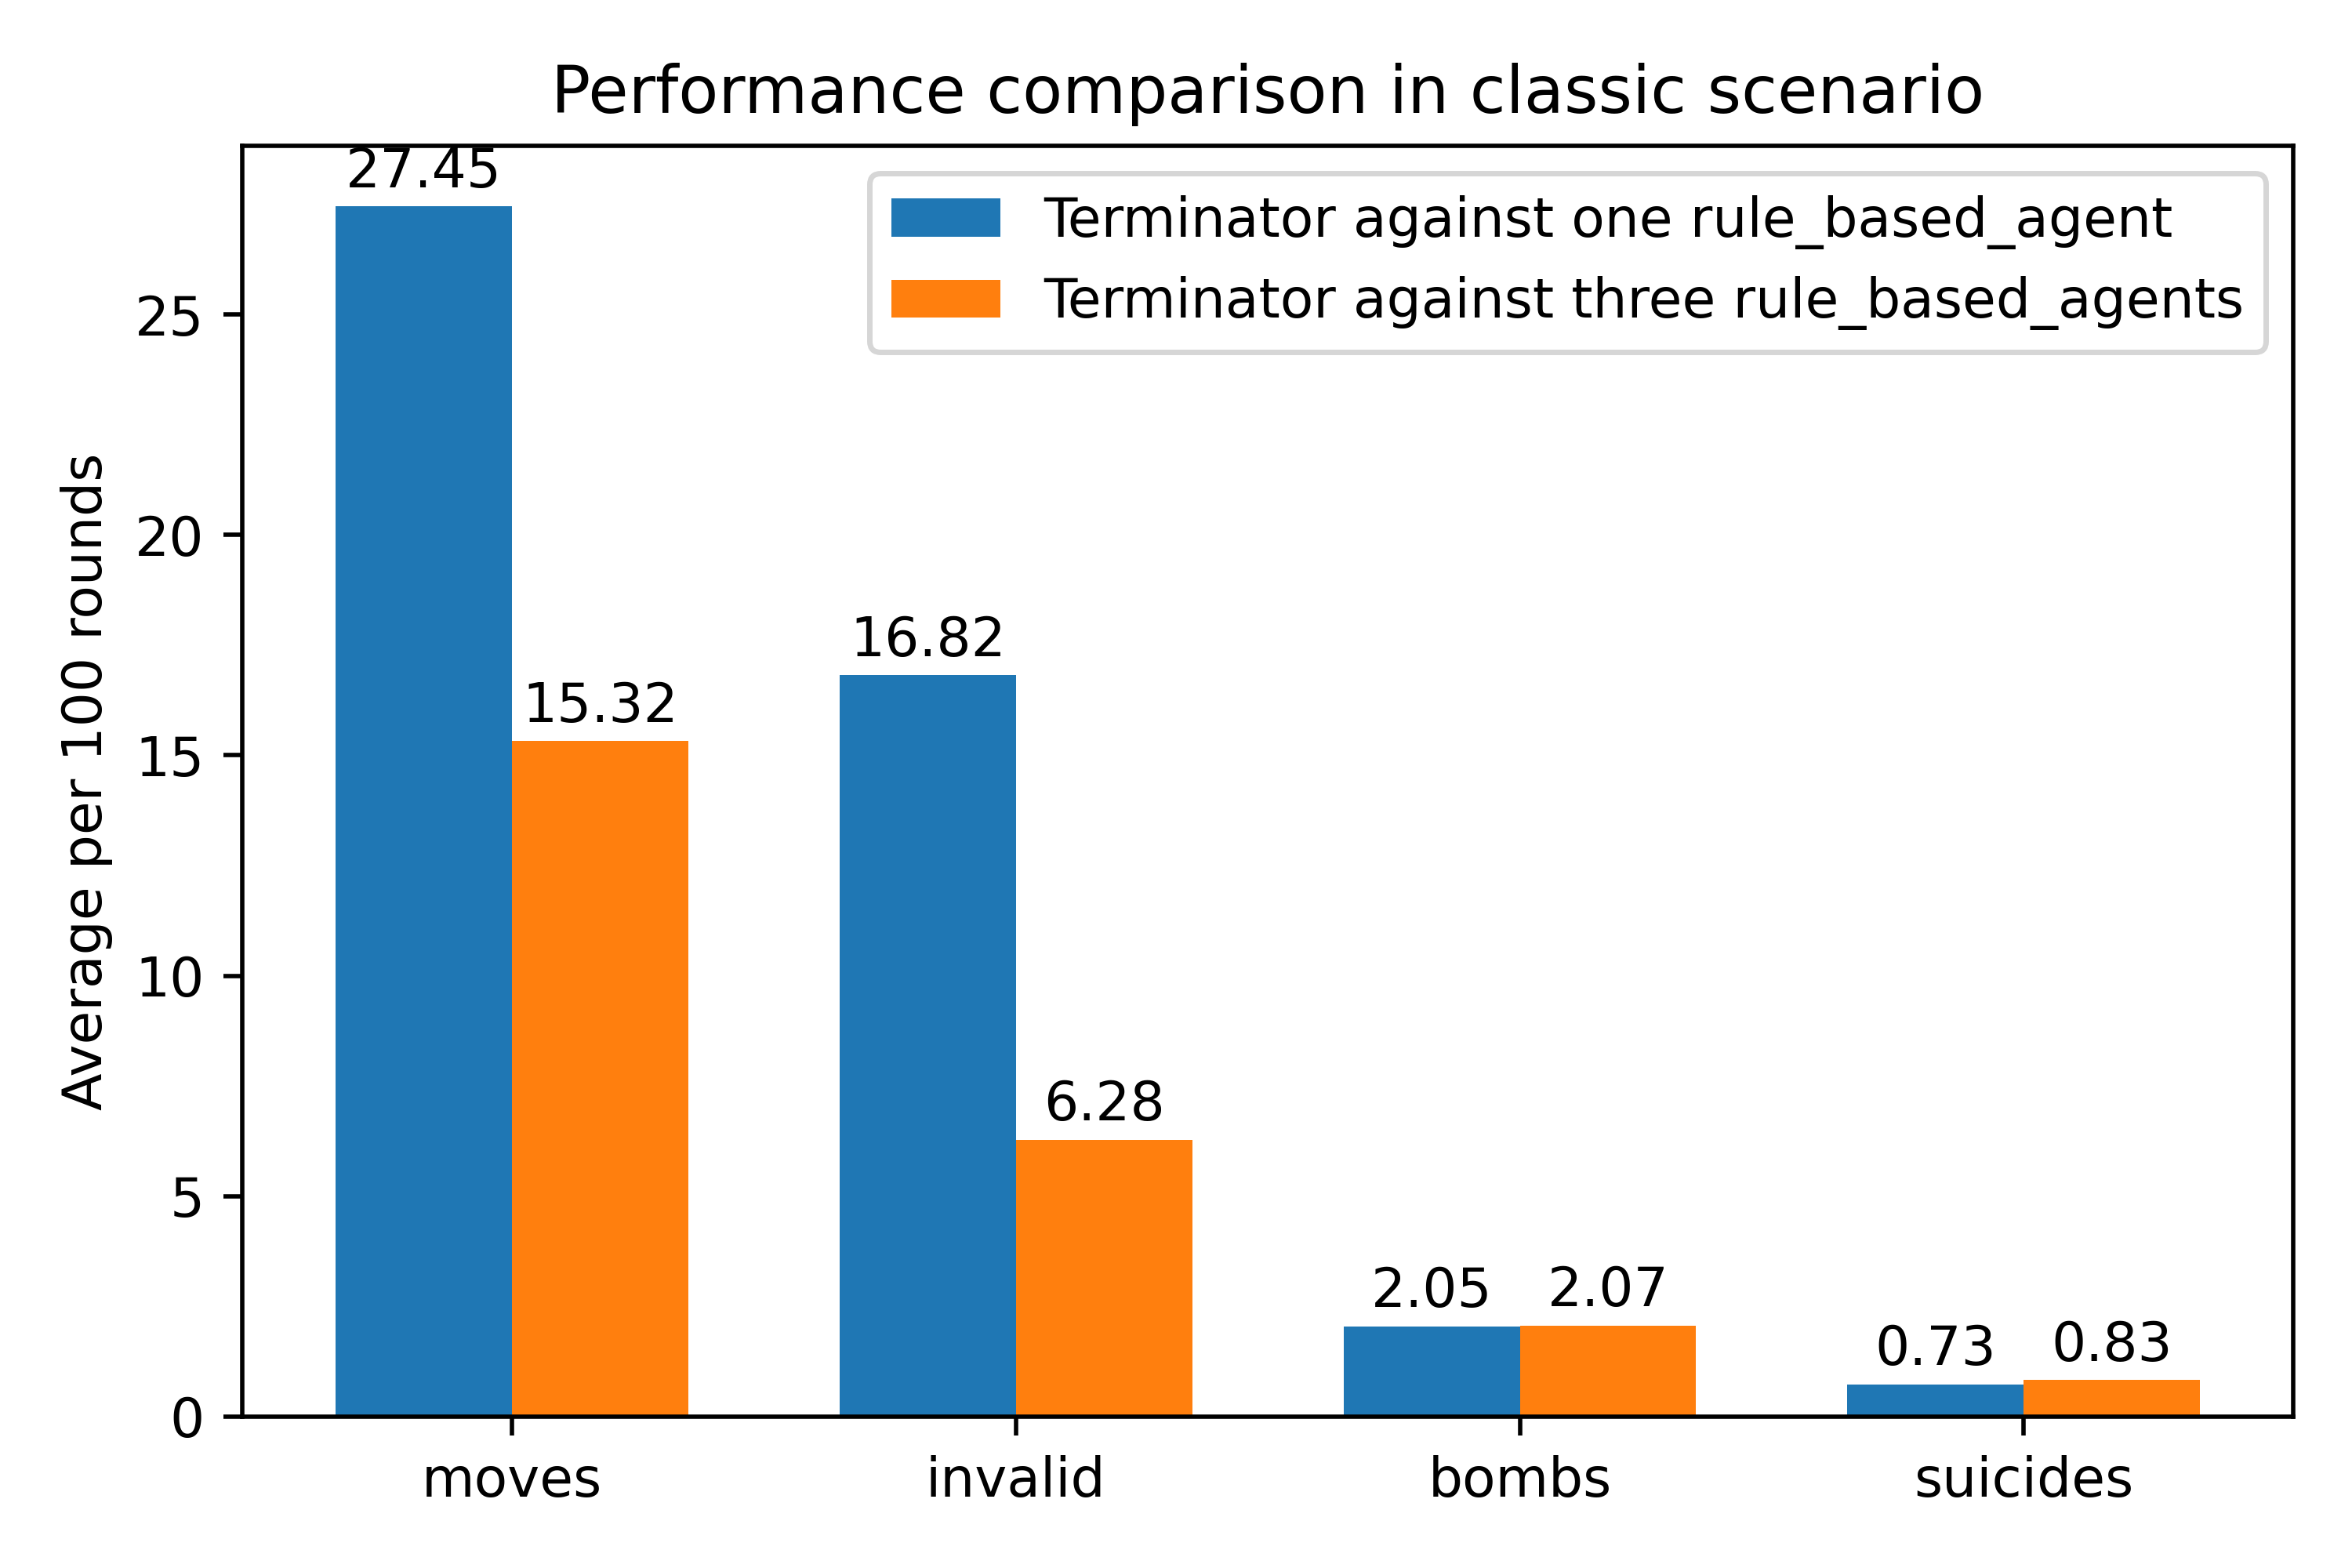
\includegraphics[scale=0.6]{Figures/Task4-1.png}
		\caption{Performance comparison Terminator against one rule\_based\_agent and three against rule\_based\_agents moves}
		\label{img:Task4-1}
	\end{subfigure}

	\begin{subfigure}{\textwidth}
		\centering
		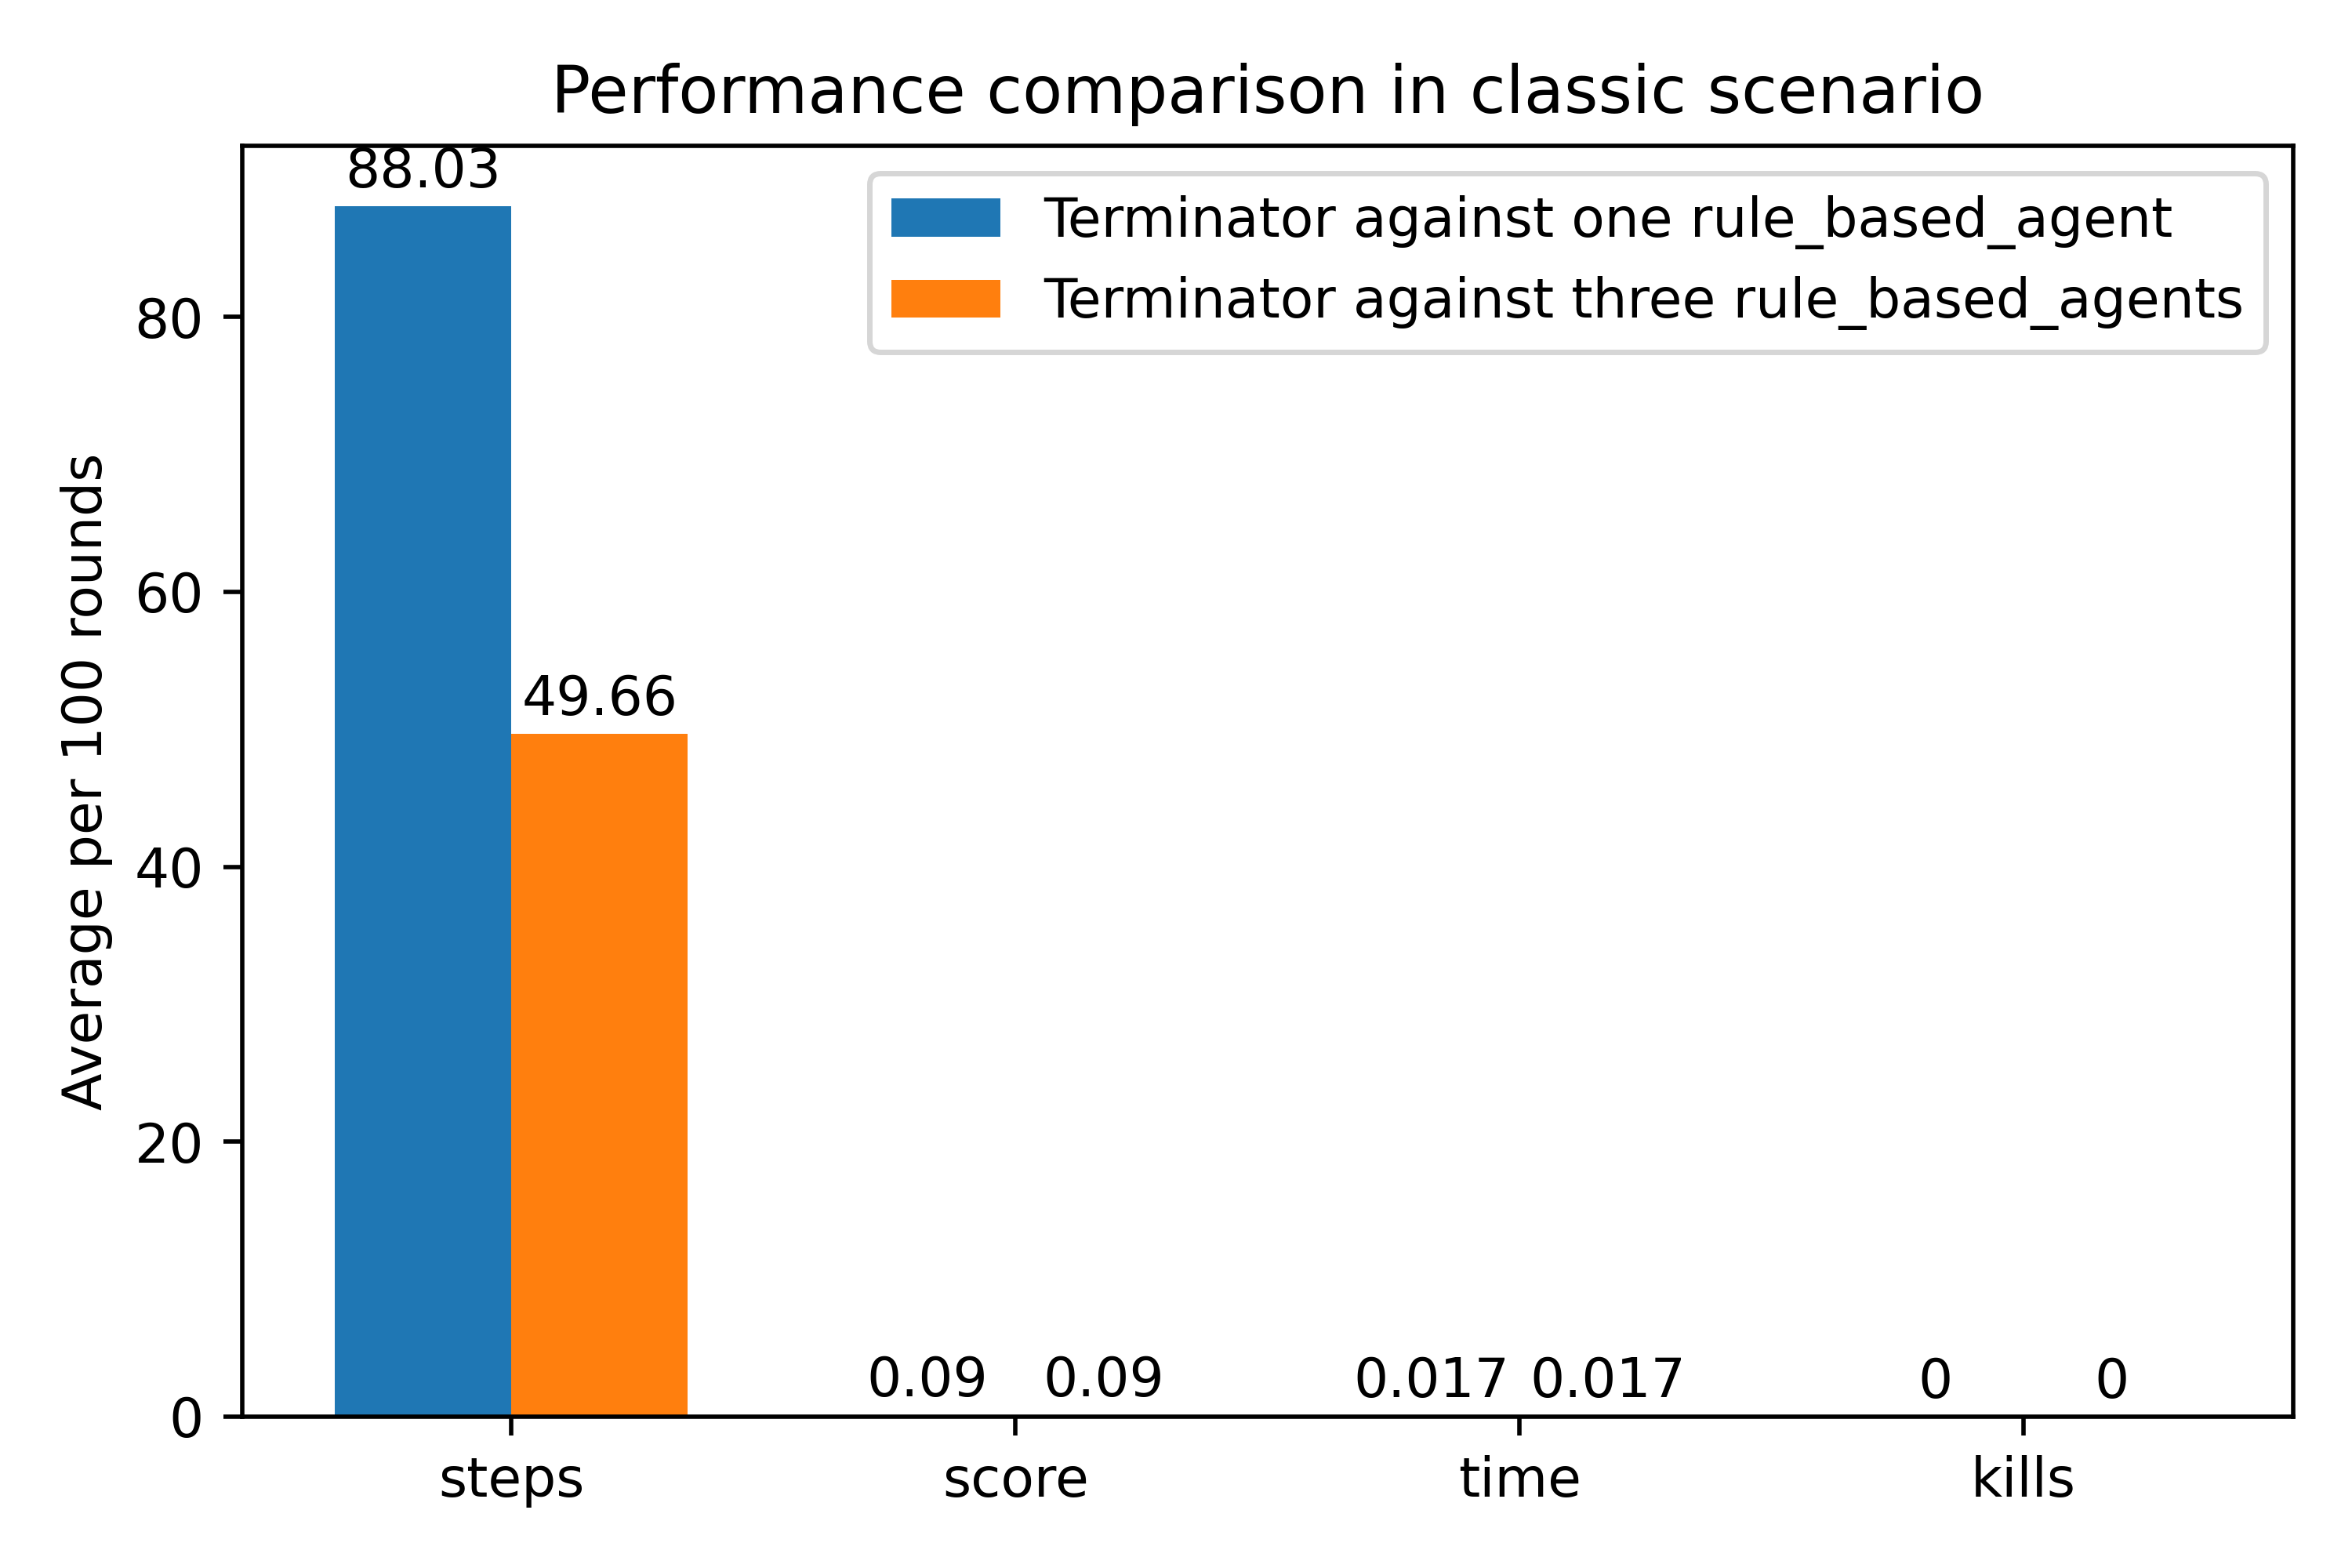
\includegraphics[scale=0.6]{Figures/Task4-2.png}
		\caption{Performance comparison Terminator against one rule\_based\_agent and three against rule\_based\_agents game}
		\label{img:Task4-2}
	\end{subfigure}

	\caption{Performance comparison Terminator against one rule\_based\_agent and three against rule\_based\_agents}
	\label{img:Task4}

\end{figure}

Figure \ref{img:Task3-1} and \ref{img:Task3-2} compare the performance of Terminator against one rule\_based\_agent and against three rule\_based\_agent.
The rule\_based\_agent not only tries to collect coins but also to kill other opponents.
Terminator has a hard time surviving against the rule\_based\_agent.
With three rule\_based\_agent in the game he dies significantly faster than with only one.
Interestingly the score is the same in both cases.
This might be caused by the agent collecting a coin before an other agent can even kill him.
Other than that he still did not manage to kill an opponent.

%----------------------------------------------------------------------------------------
%	CONCLUSION
%----------------------------------------------------------------------------------------

\section{Conclusions}


\subsection*{Q-Learning}


%----------------------------------------------------------------------------------------
%	BIBLIOGRAPHY
%----------------------------------------------------------------------------------------

\printbibliography % Output the bibliography

%----------------------------------------------------------------------------------------

\end{document}